%%%%%%%%%%%%%%%%%%%%%%%%%%%%%%%%%%%
% Basic formatting and settings
%%%%%%%%%%%%%%%%%%%%%%%%%%%%%%%%%%%
\documentclass[12pt,a4paper]{report}
\usepackage[utf8x]{inputenc}
\usepackage[IL2]{fontenc}
\usepackage{a4wide}
\usepackage[left=2cm, right=2cm, top=2.5cm, bottom=2.5cm]{geometry}

%%%%%%%%%%%%%%%%%%%%%%%%%%%%%%%%%%%
% Include required packages
%%%%%%%%%%%%%%%%%%%%%%%%%%%%%%%%%%%
\usepackage{amsmath,amssymb,amsthm}
\usepackage[usenames]{color}
\usepackage{nicefrac}
\usepackage{verbatim}
\usepackage{graphicx}
\usepackage{enumitem}
\usepackage{setspace}
\usepackage{tabularx}
\usepackage{listings}
\usepackage[section]{placeins}

\usepackage[pdftex,bookmarks=true,colorlinks,linkcolor=blue,urlcolor=blue,unicode]{hyperref}
\hypersetup{pdftitle=ODCleanStore}

%%%%%%%%%%%%%%%%%%%%%%%%%%%%%%%%%%%
% Additional formatting settings
%%%%%%%%%%%%%%%%%%%%%%%%%%%%%%%%%%%

%\pagestyle{plain}
\pagestyle{headings}
\linespread{1.1}
\setcounter{secnumdepth}{3}
\setcounter{tocdepth}{2}

%%%%%%%%%%%%%%%%%%%%%%%%%%%%%%%%%%%
% Include macro definitions and package settings
%%%%%%%%%%%%%%%%%%%%%%%%%%%%%%%%%%%

%%%%%%%%%%%%%%%%%%%%%%%%%%%%%%%%%%%
% Indent settings for paragraphs, itemize and enumerate environment
%%%%%%%%%%%%%%%%%%%%%%%%%%%%%%%%%%%
\setitemize{noitemsep,topsep=2pt,leftmargin=30pt}
\setenumerate{noitemsep,topsep=2pt,leftmargin=30pt}
\setdescription{style=sameline}
%\setlength{\parindent}{0pt} % nastavuje odsazení prvniho radku
%\setlength{\parskip}{1.2ex plus 0.5ex minus 0.2ex} % odstup mezi odstavci

\newcommand{\moreindent}{\addtolength{\leftskip}{1.8em}}
\newcommand{\lessindent}{\addtolength{\leftskip}{1.8em}}
\newcommand{\suppressgaps}{\setlength{\parskip}{0pt}}

%%%%%%%%%%%%%%%%%%%%%%%%%%%%%%%%%%%
% Shortcuts for math mode
%%%%%%%%%%%%%%%%%%%%%%%%%%%%%%%%%%%
\newcommand{\coloneqq}{\mathrel{\mathop:}=}
\renewcommand{\O}{{\mathcal{O}}}
\newcommand{\etc}[2]{#1_1,\ldots,#1_#2}
\def\<#1>{\leavevmode\hbox{\it #1\/}} % usage: \<variable>

%%%%%%%%%%%%%%%%%%%%%%%%%%%%%%%%%%%
% Other shortcuts and style commands
%%%%%%%%%%%%%%%%%%%%%%%%%%%%%%%%%%%
\newcommand{\quot}[1]{``#1''}
\newcommand{\code}[1]{\texttt{#1}}
\newcommand{\varcode}[1]{\textit{\textless #1\textgreater}}
\newcommand{\vartext}[1]{\textit{#1}}
\newcommand{\tab}{\rule{30pt}{0pt}}
\newcommand{\term}[1]{\textit{#1}}
\newcommand{\todo}[1]{}
\newcommand{\importantterm}[1]{\textbf{#1}}

% These macros use a dirty trick to persuade LaTeX to typeset chapter headers
% more readably and not to leave plenty of space above them.
\makeatletter
\def\@makechapterhead#1{
  {\parindent \z@ \raggedright \normalfont
   \Huge\bfseries \thechapter. #1
   \par\nobreak
   \vskip 20\p@
}}
\def\@makeschapterhead#1{
  {\parindent \z@ \raggedright \normalfont
   \Huge\bfseries #1
   \par\nobreak
   \vskip 20\p@
}}
\makeatother

% Chapter that is not numbered but included in the contents
\def\chapwithtoc#1{
\chapter*{#1}
\addcontentsline{toc}{chapter}{#1}
} 

\newenvironment{enumeratei}
	{
		\begin{enumerate}
		\renewcommand{\labelenumi}{(\textit{\roman{enumi}})}
	}
	{
		\end{enumerate}
	}

\newenvironment{glossarylist}
	{\begin{description}[style=nextline,itemsep=8pt]}
	{\end{description}}

\newenvironment{configlist}
	{\begin{description}[style=nextline,font=\ttfamily]}
	{\end{description}}

\newenvironment{dirlist}
	{\begin{description}[style=sameline,font=\ttfamily]}
	{\end{description}}
	
%%%%%%%%%%%%%%%%%%%%%%%%%%%%%%%%%%%
% Package settings
%%%%%%%%%%%%%%%%%%%%%%%%%%%%%%%%%%%%

% lstlistings environment
% Defines a custom trivlisting environment
\lstset{basicstyle=\ttfamily\footnotesize,columns=flexible,
  frame=lines,float=ht,captionpos=b,aboveskip=1.5\bigskipamount}
\lstnewenvironment{trivlisting}
  {\lstset{basicstyle=\ttfamily,aboveskip=\medskipamount,frame=none}}
  {}

%%%%%%%%%%%%%%%%%%%%%%%%%%%%%%%%%%%
% Document-specific commands
%%%%%%%%%%%%%%%%%%%%%%%%%%%%%%%%%%%
\newcommand{\refusermanual}{User Manual\xspace}
\newcommand{\refadminmanual}{Administrator's \& Installation Manual\xspace}
\newcommand{\refprogrammersguide}{Programmer's Guide\xspace}
\newcommand{\configdefault}[1]{\newline\textit{Default value:}~\code{#1}}
\newcommand{\odcs}{ODCleanStore\xspace}
\newcommand{\reqparagraph}[1]{\paragraph{\textnormal{\textit{#1}}}}

%%%%%%%%%%%%%%%%%%%%%%%%%%%%%%%%%%%
% Aligned enumeration tables
%%%%%%%%%%%%%%%%%%%%%%%%%%%%%%%%%%%
\newcommand{\enumtable}[1]
{
	\begin{table}[!ht]
		\begin{tabularx}{\linewidth}{>{\textbf\bgroup}l<{\egroup}X}
			#1
		\end{tabularx}
	\end{table}
}

%%%%%%%%%%%%%%%%%%%%%%%%%%%%%%%%%%%
% Aligned field description tables
%%%%%%%%%%%%%%%%%%%%%%%%%%%%%%%%%%%
\newcommand{\fieldtable}[1]
{
	\begin{table}[!ht]
		\begin{tabularx}{\linewidth}{|>{\textbf\bgroup}l<{\egroup}|p{3cm}|X|}
			\hline
			\textnormal{Required} & Field & Description \\
			\hline \hline
			#1 \\
			\hline
		\end{tabularx}
	\end{table}
}


%%%%%%%%%%%%%%%%%%%%%%%%%%%%%%%%%%%
% Optionally disable use of images.
% Convenient for export to .dvi when the documents contain images not supported in plain latex
% Uncomment to disable images.
%%%%%%%%%%%%%%%%%%%%%%%%%%%%%%%%%%%
%\renewcommand{\includegraphics}[2][1]{}

\newcommand{\version}{0.3.7}
\newcommand{\documentname}{\refusermanual}

\hypersetup{pdftitle=ODCleanStore -- \documentname}

\begin{document}

\title{ODCleanStore -- \documentname}

\begin{titlepage}
\begin{center}

\large
Charles University in Prague

\smallskip

Faculty of Mathematics and Physics

%\vspace{\stretch{1}}
%{\bf\Large SOFTWARE PROJECT}

\vspace{\stretch{3}}

\resizebox{0.5\linewidth}{!}{\bf\Huge ODCleanStore}

%\bigskip
%\resizebox{0.3\linewidth}{!}{Open Data store}

\vspace{\stretch{3}}
\begin{spacing}{1.5} 
{\bf\Huge \documentname}
\end{spacing}

\vspace{\stretch{1}}
Release \version\\
\today

\vspace{\stretch{15}}

\begin{tabular}{rl}

\textbf{Authors:} & Jan Michelfeit \\
& Du\v san Rychnovsk\'y\\
& Jakub Daniel\\
& Petr Jerman\\
& Tom\' a\v s Soukup\\
\noalign{\vspace{3mm}}
\textbf{Supervisor:} & RNDr. Tom\' a\v s Knap
\end{tabular}

\end{center}
\end{titlepage}

\newpage

\renewcommand{\contentsname}{Contents}
\tableofcontents
\bigskip

\newpage

%%%%%%%%%%%%%%%%%%%%%%%%%%%%%%%%%%%%%%%%%%%%%%%%%%%%%%%%%%%%%%%%%%%%%%%%%%%%%%

\chapter{Introduction}
\label{chap:introduction}

The advent of Open Data\footnote{\url{http://opendatahandbook.org/}} and Linked Data\footnote{\url{http://www.w3.org/standards/semanticweb/data}; \url{http://linkeddata.org/}}  accelerates the evolution of the Web into an exponentially growing information space\footnote{See the Linked Open Data Cloud at \url{http://richard.cyganiak.de/2007/10/lod/}} where the unprecedented volume of data will offer information consumers a~level of information integration and aggregation agility that has up to now not been possible. Data consumers can now \quot{mashup} and readily integrate information in myriads of applications.

Indiscriminate addition of information, however, comes with inherent problems, such as the provision of poor quality, inaccurate, irrelevant or fraudulent information. All will come with an associate cost of the data integration which will ultimately affect data consumer's benefit and Linked Data applications usage and uptake.

To overcome these issues, we present a~framework enabling management of Linked Data -- data cleaning, linking, transformation and quality assessment -- and providing  applications with a~possibility to consume the stored cleaned and integrated data, which reduces the costs of application development.

\section{What is ODCleanStore}

In short, ODCleanStore is a~server application for management of Linked Data -- it stores data in RDF, processes them and provides integrated views on the data.

ODCleanStore accepts arbitrary RDF data through a~webservice (together with provenance and other metadata). The data is processed by \term{transformers} in one of a~set of customizable \term{pipelines} and stored to a~persistent store. The stored data can be accessed again through a~webservice. Linked Data consumers can send queries and custom query policies to this webservice and receive (aggregated/integrated) RDF data relevant for their query, together with information about provenance and data quality. Overview of ODCleanStore is depicted on \figurename~\ref{fig:odcsInternal}.

ODCleanStore is developed at the Charles University in Prague, Faculty of Mathematics and Physics as part of the \href{http://opendata.cz}{OpenData.cz} initiative and the \href{http://lod2.eu}{LOD2.eu} project and published as a~free software under Apache License 2.0. The project is hosted at SourceForge at
\begin{center}
  \url{http://sourceforge.net/p/odcleanstore/}.
\end{center}

\begin{figure}[htb]
    \centering
    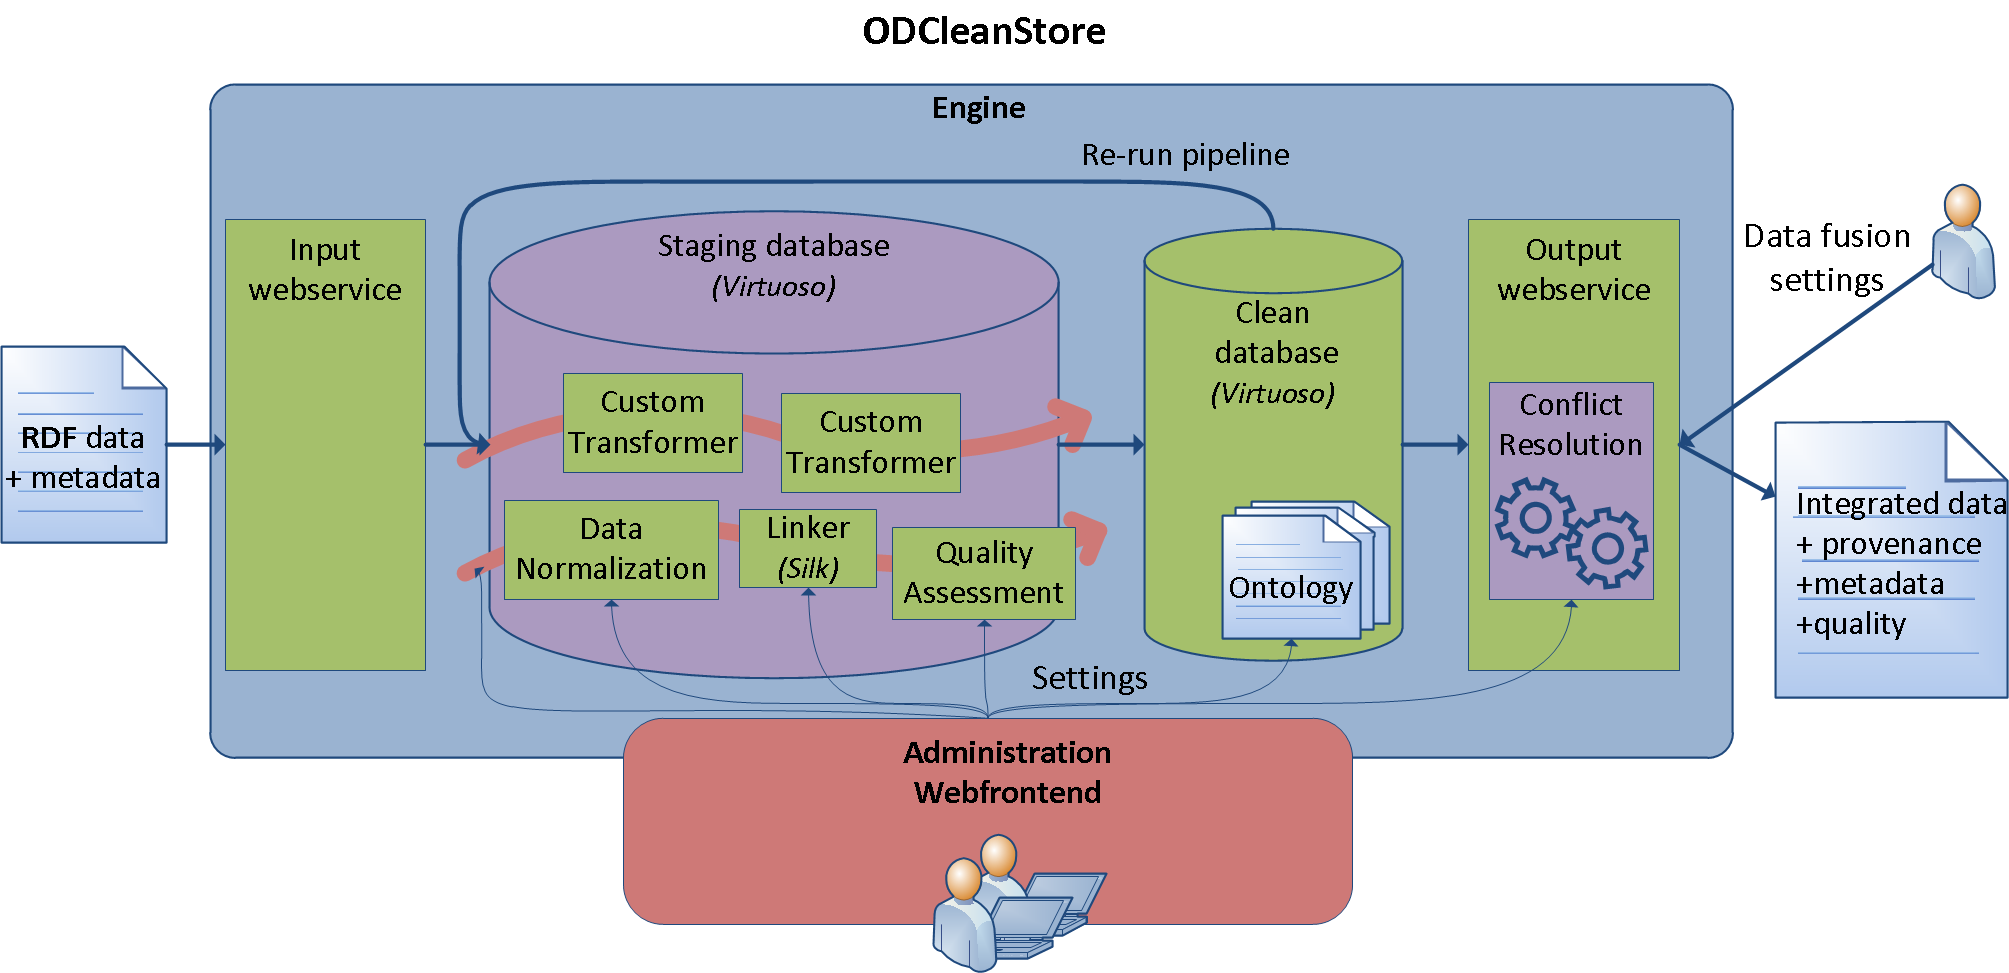
\includegraphics[width=\textwidth]{images/odcs-internal.png}
    \caption{Overview of ODCleanStore architecture}
	\label{fig:odcsInternal}
\end{figure}

\section{How to Read This Document}

This document is a~user manual with basic description od ODCleanStore and detailed instructions on how to access and work with the application from the perspective of a~user. Chapters \ref{chap:introduction} and \ref{chap:howItWorks} give a~basic description of what ODCleanStore is and how it works, while Chapter \ref{chap:userRoles} describes user roles and will guide you to other parts of this manual relevant for your user role.

If more detailed information is needed, please refer to related documents \quot{\refadminmanual} and \quot{\refprogrammersguide}.

\todo{what is important, what is different from others, how do we support the goals}

\section{Linked Data Framework}

The goal of the \href{http://opendata.cz}{OpenData.cz} initiative is to build an open data infrastructure in The Czech Republic. It would provide public data in a~form that allows access to anyone at any time and allows to combine it freely. This would allow the creation of applications that the public really needs.

ODCleanStore is a~part of the Linked Data Framework developed under the OpenData.cz initiative. The main three parts of the framework are \term{Data Acquisition} module, \term{Data Aggregation and Cleaning} module and \term{Data Visualization and Analysis} module.

\todo{picture}

The Data Acquisition module\footnote{\url{http://strigil.sourceforge.net/}} will be able to crawl webpages and scrape structured data from webpages and other sources (such as XLS spreadsheets). This data is converted to RDF and sent to the Data Aggregation and Cleaning module represented by ODCleanStore. ODCleanStore processes the data, stores it and provides access to it. The Visualization and Analysis module will query ODCleanStore and provide a~human-friendly interface to end users.


\section{Examples of Deployment}

ODCleanStore is planned to be deployed together with the Data Acquisition module represented by project Strigil\footnotemark[\thefootnote] which would feed up-to-date data to ODCleanStore. However, thanks to the use of standard formats for communication with the input/output webservices, ODCleanStore can be deployed with any other third-party application for data feeding or consuming.

In general, ODCleanStore is intendend to be used whenever there are multiple sources of (semi-)structured data convertible to RDF that need to be integrated. ODCleanStore can be used for academic purposes, \quot{mashup} applications, or even deployed in an enterprise environment.

A real-world deployment is planned for storing public contracts data published by the public administration of the Czech Republic as part of the OpenData.cz initiative. Another deployment will be for internal use in students' projects at the Charles University in Prague.

%%%%%%%%%%%%%%%%%%%%%%%%%%%%%%%%%%%%%%%%%%%%%%%%%%%%%%%%%%%%%%%%%%%%%%%%%%%%%%

\chapter{How It Works}
\label{chap:howItWorks}

ODCleanStore consists of \term{Engine}, \term{Input Webservice} and \term{Output Webservice} (both run as part of the Engine), and administration webfrontend. The Engine processes incoming and stored data using \term{transformers}. A~transformer is a~pluggable Java class implementing a~defined interface; several transformers ship with ODCleanStore, such as Quality Assessment, Linker or Data Normalization.

\section{Data Lifecycle}

The lifecycle of data inside ODCleanStore is as follows:

\begin{enumerate}
  \item RDF data (and additional metadata) are accepted by Input Webservice and stored as a~named graph to the \term{dirty database}. Data can be uploaded by any third-party application registered in ODCleanStore.
  \item Engine successively processes named graphs in the dirty database by applying a~pipeline of transformers to it; the applied pipeline is selected according to the input metadata.
  \item Each transformer in the pipeline may modify the named graph or attach new related named graphs (such as a named graph with mappings to other resources or results of quality assessment).
  \item When the pipeline finishes, the augmented RDF data are populated to the \term{clean database} together with any auxiliary data and metadata created during the pipeline execution.
  \item Data consumers can use Output Webservice to query data in the clean database. Output Webservice provides several basic types of queries -- URI query, keyword and named graph query; in addition, metadata about a~given named graph can be requested. The response to a~query consists of relevant RDF triples together with their provenance information and quality estimate. The query can be further customized by user-defined conflict resolution policies.\\
	Data in the clean database can be also queried using the SPARQL query language. While SPARQL queries are more expressive, there is no direct support for provenance tracking and quality estimation. 
  \item When transformer rules change, the administrator may choose to re-run a~pipeline on data already stored in the clean database. Copy of this data is created in the dirty database where it is processed by the pipeline. After that, the processed version of data replaces the original in the clean database.
\end{enumerate}

\section{Administration Frontend Features}
The administration webfrontend enables
\begin{itemize}
  \item management of user accounts,
  \item management of pipelines, transformers and transformer rules,
  \item management of ontologies,
  \item monitoring of inserted data and the state of Engine,
  \item management of other settings, such as default conflict resolution policies for queries.  
\end{itemize}

\section{Summary of Features}

\begin{itemize}
  \item Administration in a~simple web interface.
  \item Input and Output Webservices communicate in standard formats - Input Webservice accepts RDF/XML or TTL, Output Webservice provides results in HTML, TriG and RDF/XML formats.
  \item Highly customizable pipelines for incoming data processing. Different pipelines can be used for different data sources.
  \item Data can be processed before they are stored to a~persistent store but also when they are already stored if neccessary.
  \item Ships with several predefined transformers for use in data-processing pipelines: Data Normalization (transformations of data), Quality Assesment (estimates quality of data based on a~set of rules), Linker (links RDF resources representing the same entity or otherwise related). All these transformers can be managed in the web administration interface.
  \item Support for ontology management. Mappings between ontologies can be defined in order to integrate heterogeneous data. Also, rules for  transformers can be automatically generated from ontologies.
  \item Data consumers can query for all data about a~given resource or use the keyword search.
  \item Response to a~query includes provenance information and quality estimate of each RDF triple in the result. More provenance metadata can be requested. Conflicts that arise when integrating data are solved at query time according to user-defined policies. 
\end{itemize}


%%%%%%%%%%%%%%%%%%%%%%%%%%%%%%%%%%%%%%%%%%%%%%%%%%%%%%%%%%%%%%%%%%%%%%%%%%%%%%

\chapter{User Roles}
\label{chap:userRoles}

Data consumers accessing Output Webservice (see Section~\ref{sec:outputWS}) do not need to have an account in ODCleanStore; these users have a~special role User (USR). Other users working with ODCleanStore need to have an account and their permissions are based on the roles they are assigned. This chapter describes all the roles recognized by ODCleanStore.

\begin{figure}[!htb]
    \centering
    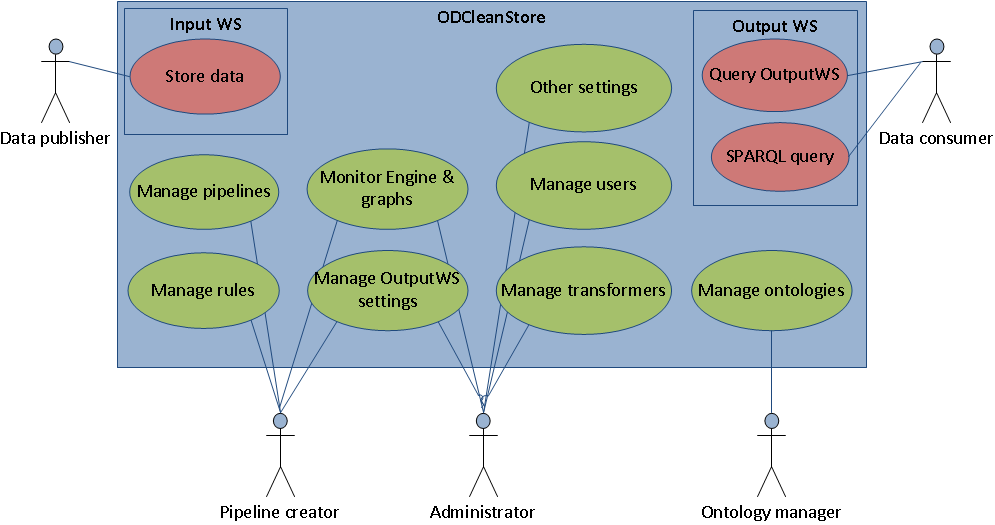
\includegraphics[width=\textwidth]{images/use-cases.png}
    \caption{Overview of roles in ODCleanStore}
	\label{fig:odcsUseCases}
\end{figure}

\section[Administrator]{Administrator (ADM)}
\label{sec:adm}

	Administrator has privileges to manage user accounts, assign roles and manage system-wide settings such as
	\begin{itemize}
		\item transformers that can be used in pipelines created by pipeline creators,
		\item settings of Output Webservice (default aggregation policies, etc.),
		\item URI prefixes that can be used in settings and queries.
	\end{itemize}

	In addition, the administrator is authorized to edit pipelines and rules created by pipeline creators.

% TODO Tohle bych dal do admin manualu, ma to na starost administrator ODCS jako takovy, coz neni nutne uzivatel s roli ADM:
%	The administrator is responsible for ensuring that not more than one instance of the storage and its web frontend is connected to one instance of database.


	More information, e.g. about adding transformers, can be found in the related document \refadminmanual.

	\paragraph{Most relevant sections of this document:} Chapter \ref{chap:administrationFrontend} \nameref{chap:administrationFrontend}.

\section[Ontology Creator]{Ontology Creator (ONC)}
\label{sec:onc}
	The ontology creator can import and edit ontologies registered in the system. The ontology creator is also responsible for inserting mappings (\code{owl:sameAs} links) between ontologies.

	\paragraph{Most relevant sections of this document:} Section \ref{sec:ontologyManagement} \nameref{sec:ontologyManagement}.

\section[Pipeline Creator]{Pipeline Creator (PIC)}
\label{sec:pic}
	The pipeline creator can create input data processing pipelines. This includes creating new pipelines, assigning transformers to them (Section \ref{sec:pipelineManagement}) and also creating rules for the transformers (Section \ref{sec:transformerRules}). In addition, pipeline creator can monitor state of graphs sent to ODCleanStore and errors that occur during pipeline processing (Section \ref{sec:engineState}).

	Every pipeline creator is allowed to create custom pipelines and rule groups for predefined transformers. The pipeline creator has a~read-only access to other creators' pipelines and rules (and can use such rules in custom pipelines), however rules and pipelines can only be edited by their author. The only exception is the administrator, who can edit arbitrary pipelines and rule groups.

	 The same principle applies for inserted graphs management -- pipeline creator can delete or re-run pipeline for graphs that were processed by a pipeline created by this pipeline creator, while administrators are authorized for manipulation with all graphs.

	\paragraph{Most relevant sections of this document:} Sections \ref{sec:pipelineManagement} \nameref{sec:pipelineManagement},\linebreak[4] \ref{sec:transformerRules} \nameref{sec:transformerRules}, \ref{sec:engineState} \nameref{sec:engineState} and \linebreak[4] \ref{sec:pipelinesOnCleanDB} \nameref{sec:pipelinesOnCleanDB}.
	
\section[Data Producer]{Data Producer (SCR)} \todo{SCR? DAP?}
\label{sec:scr}
  The data producer can use Input Webservice (Section \ref{sec:inputWS}) to insert new data to ODCleanStore. The system keeps track of which data were inserted by which data producer.

  \paragraph{Most relevant sections of this document:} Sections \ref{sec:inputWS} \nameref{sec:inputWS} and \linebreak[4] \ref{sec:inputProcessing}~\nameref{sec:inputProcessing}.

\section[Data Consumer]{Data Consumer (USR)} \todo{USR? DAC?}
\label{sec:usr}
  The data consumer can use Output Webservice (Section \ref{sec:outputWS}) to ask queries over the data in the clean database. This role is special in that users in this role do not need to have an account (any user using the Output Webservice is automatically assigned the USR role).

  \paragraph{Most relevant sections of this document:} Sections \ref{sec:outputWS} \nameref{sec:outputWS} and \linebreak[4] \ref{sec:storedDataStructure}~\nameref{sec:storedDataStructure}.

%%%%%%%%%%%%%%%%%%%%%%%%%%%%%%%%%%%%%%%%%%%%%%%%%%%%%%%%%%%%%%%%%%%%%%%%%%%%%%

\chapter{Administration Frontend}
\label{chap:administrationFrontend}

\section{Administration Frontend Overview}

Administration Frontend is the tool for managing ODCleanStore. It covers configuration of all standard components. It is restricted to authorized users only. 

The administration frontend controls various entities, allows the user to set different attributes and perform actions on those entities. Several terms and designations are used repeatedly in the frontend, however, their meanings do not change, therefore make sure to be familiar with them as they might not be described hereafter.

\subsection*{Common attributes}

\enumtable
{
	\vspace{0.5cm} Label & A unique human readable identifier of the related entity.\\
	\vspace{0.5cm} Description & A description for user's purposes and better comprehension of semantics of the related entity.\\
	\vspace{0.5cm} Author & The username of a the originator / creator of the related entity.
}

\subsection*{Common actions}

\enumtable
{
	\vspace{0.5cm} Delete & Remove the related entity irrevertably from the system.\\
	\vspace{0.5cm} Detail & View details and form for editing the related entity. For some entitis shows also entities related to the edited entity.\\
	\vspace{0.5cm} Rerun affected graphs & Queues all graphs affected by the entity for pipeline processing, i.e. the graphs will be processed again by their respective pipeline.
}

The frontend is divided into several separate sections of logicaly related controls. The main menu bar at the top of the page can be used to switch between those sections.

\begin{figure}[tb]
    \centering
    
\includegraphics[width=\textwidth]{images/fe-main-menu-bar.png}
    \caption{Main menu}
	\label{fig:feHome}
\end{figure}

\begin{figure}[tb]
    \centering
    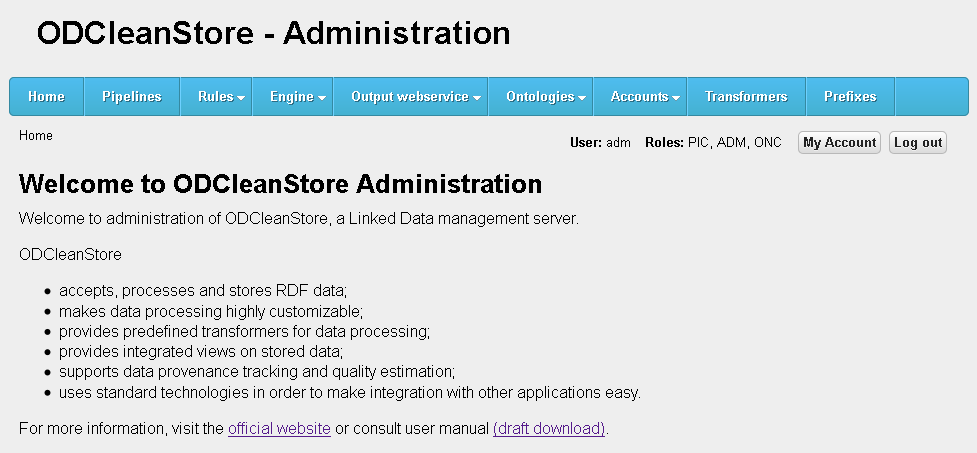
\includegraphics[width=\textwidth]{images/fe-home-screenshot.png}
    \caption{Administration Frontend after login}
	\label{fig:feHome}
\end{figure}

\section{Pipeline Management}
\label{sec:pipelineManagement}

	New incoming data (in form of a named graph) accepted by Input Webservice are passed through a {pipeline} consisting of {transformers}. In this section of the administration frontend it is possible for the user to specify different {pipelines}. Individual {pipelines} can incorporate different already existing {transformers}. To edit the structure of a {pipeline}, view its detail.

\begin{figure}[tb]
    \centering
    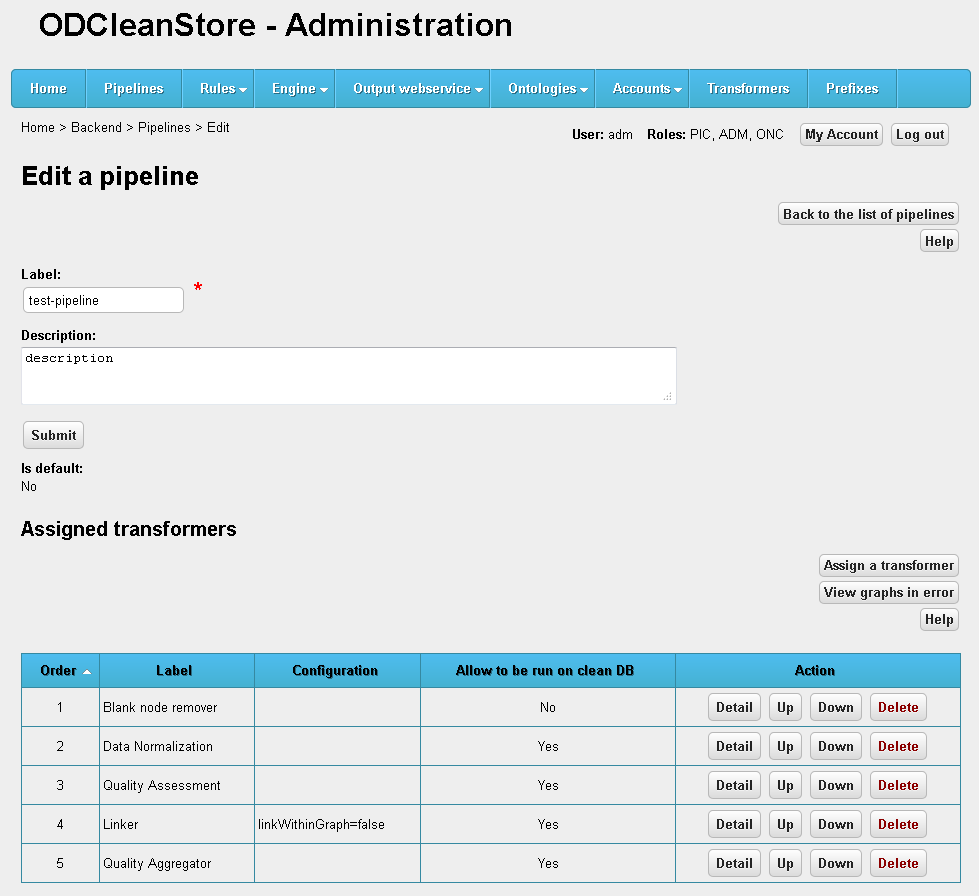
\includegraphics[width=\textwidth]{images/fe-pipeline-screenshot.png}
    \caption{Pipeline editing}
	\label{fig:feHome}
\end{figure}

\subsection*{Individual Transformer Instances}

	In a detail page of any particular pipeline there is a list of transformers assigned to it. Each assignment composes of these fields:

	\fieldtable
	{
		required & transformer/label & an existing transformer label\\
		\hline
		required & working dir & an existing directory designated to the above selected transformer\\
		\hline
		required & configuration & configuration passed to an instance of the above selected transformer\\
		\hline
		implied & allow to be run on clean DB & As the importance of data modification that the pipelines can cause differs based on what database it is running upon, it is left for the user to decide whether a concrete {transformer} should be allowed to run on clean database (in addition to running on dirty database). Some transformations do not even make sense when working with clean database.\\
		\hline
		required & place in pipeline before & Determines when the transformer will be run in respect to other transformers in the pipeline
	}

	The detail page of the assigned \QA, \DN, \OI transformers allows user to specify what rule groups are assigned to the transformer in the related pipeline.

%\paragraph{Important note:} Any changes done in this section need to be commited to ever take effect. To do so, please, click the \quot{Commit settings} button.
% TODO: the previous paragraph is outdated, to be replaced by commiting of rules within a single group

\subsection{Predefined Transformers}
Several transformers are included in ODCleanStore by default. This section provides their overview.

\subsubsection{Quality Assessment}

This transformer assigns a quality indicator to the processed named graph based on data properties contained in it. It will be further described in section \ref{sub:qualityAssessment}.

\subsubsection{Quality Aggregator}

This transformer assigns a quality indicator to the publisher of the processed named graph based on quality of all graphs stored in the database and sharing this publisher. It will be further described in section \ref{sub:qualityAssessment}.

\subsubsection{Data Normalization}

This transformer can be used to modify data contained in the processed graph. The main reason to allow modifications is to be able to cope with situations when data from different sources have different forms. It is also useful to preprocess data to better suit the rest of the transformation process and future queries of other users. For more information, see section \ref{sub:dataNormalization}.

\subsubsection{Linker}
% TODO
Purpose of this transformer is to identify related information and create links that represent the relation. To find out how to control this transformer see section \ref{sub:objectIdentification}.

\subsubsection{Blank Node Remover}
This transformer replaces all blank nodes in \code{payload} named graph with unique URI resources. The transformer guarantees that occurrences of the same blank node withing the transformed graph (and only this graph) will be assigned the same URI.

The URIs generated in place of blank nodes have form \varcode{prefix}\varcode{randomUUID}-\varcode{node number}. The prefix may be given in \code{Configuration} field of the transformer instance as \quot{\code{uriPrefix=}\varcode{URI prefix}} on a single line. If the prefix is not specified, the concatenation of \code{input\_ws.named\_graphs\_prefix} configuration option value and \quot{getResource} is used as the default value.

\section{Transformer Rules}
\label{sec:transformerRules}

	There are a few types of {transformers} predefined for most common data handling in pipelines. Namely:
	\begin{itemize}
		\item \term{Quality Assessessment} {transformer} (Section \ref{sub:qualityAssessment})
		\item \term{Data Normalization} {transformer}  (Section \ref{sub:dataNormalization})
		\item \term{Linker} {transformer} (Section \ref{sub:objectIdentification})
	\end{itemize}
	
	These {transformers} are configured through groups of rules. Each instance of any of these predefined {transformers} can accept multiple groups of rules. That way it is possible to simply assign all interrelated rules to a certain instance of a transformer while it is still possible to avoid duplication of rules in different groups.

\subsection{Quality Assessment}
\label{sub:qualityAssessment}

\subsubsection*{Quality Assessor}

Quality Assessor is a special {transformer} that assigns a score to each graph based on coefficients of different patterns present in the graph to reflect to what degree the data contained in it comply to a certain policy.

To be able to configure individual instances of {Quality Assessor} a group of rules needs to exist. To create one enter the Quality Assessment section reachable from Rules submenu.

Here the user can prepare groups of rules to be assigned to instances of {Quality Assessor}. Each group is identified by its label and can (and should) come with a description of its semantical significance.

On the detail page, one can specify individual rules contained in the related group. Each rule consists of a \code{GroupGraphPattern}\footnote{\url{http://www.w3.org/TR/rdf-sparql-query/\#rGroupGraphPattern}} filter, quality decrease coefficient and description, as described in Table \ref{tbl:qaFields}.

\begin{table}[!ht]
	\centering
	\begin{tabular}{|rl@{\hspace{8mm}}|c@{\hspace{8mm}}|c|}
		\hline
		& \textbf{Filter} & \textbf{Coefficient} & \textbf{Description} \\
		\hline \hline
		& \code{GroupGraphPattern} [\code{GROUP BY \ldots} [\code{HAVING \ldots}]] & $ x \in [0, 1] $ & description \\
		&&&\\
		e.g.: & \code{\{\{?s anatomy:limbs ?o\} FILTER (?o > 4)\}} & $ 0.4 $ & Too many limbs\\
		\hline
	\end{tabular}
	\caption{Quality Assessment rule fields}
	\label{tbl:qaFields}
\end{table}

Any snippet of SPARQL\footnote{\url{http://www.w3.org/TR/rdf-sparql-query/\#grammar}} to which \quot{\code{SELECT * FROM ... WHERE}} can be prepended is a valid filter and describes a property of a named graph that the author of the rule finds defective.
%%TODO: mention/omit: The use of SPARQL 1.1 features depends on underlaying Virtuoso OpenSource version.

\subsubsection*{Quality Aggregator}

Quality Aggregator is a special transformer that accumulates quality score values of all the graphs corresponding to one publisher. It then calculates an average value and assesses this aggregated quality to the publisher.

\subsection{Data Normalization}
\label{sub:dataNormalization}

\term{Data Normalizer} is a special type of {transformer} aimed to be applied early in the whole data evaluation process to simplify work of other {transformers}. Its main goal is to remove inconsistencies in forms the data is provided in.

In the Data Normalization section reachable from Rules submenu, one can prepare groups of rules to be assigned to instances of {Data Normalizer}. Each group is identified by its label and can (and should) come with a description of its semantical significance.

The detail page of a group serves the user as means of specification of individual rules contained in the selected group. Each rule is essentially a sequence of \term{SPARUL}\footnote{\url{http://www.w3.org/Submission/SPARQL-Update}} modifications put by \code{MODIFY}, \code{INSERT} and/or \code{DELETE}. New rule represents an empty sequence upon its creation.

Similarly as with the rules themselves the detail page of a rule allows the user to construct any arbitrary sequence of modifications. Components of the rule (members of the sequence) can be added by specifying their type (either \code{MODIFY}, \code{INSERT} or \code{DELETE}), modification ({SPARUL} snippet stripped off of initial \code{MODIFY} / \code{INSERT INTO} / \code{DELETE FROM} clauses); e.g.,

\begin{center}
	\code{\{?s ?p1 ?o2\} WHERE \{?s ?p1 ?o1. ?o1 ?p2 ?o2.\}}.
\end{center}

Expectedly triples (\code{?s ?p1 ?o2} in the example) are inserted into (deleted from) the current graph when the type of the component is \code{INSERT} (\code{DELETE}). Effects are immediate in respect to consecutive applications of other components of the same rule or other rules to the graph. Another example would be:

\begin{center}
	\code{\{?s ?p ?o\} WHERE \{GRAPH \$\$graph\$\$ \{SELECT ?s ?p 'Y' AS ?o WHERE \{?s ?p 1\}\}\}},
\end{center}

where \code{\$\$graph\$\$} in \code{GRAPH \$\$graph\$\$} is a place holder for name of the graph being currently processed and can be used for subqueries that need to be enclosed in \code{GraphGraphPattern}\footnote{\url{http://www.w3.org/TR/rdf-sparql-query/\#rGraphGraphPattern}}. When there is no subquery, however, it is not necessary to use the placeholder at all.

\subsection{Linker}
\label{sub:objectIdentification}

\term{Linker} is a special {trasformer}. Its main purpose is to interlink URIs which represent the same real-world entity by generating \code{owl:sameAs} links. It can be also used for creating other types of links between differently related URIs.

To be able to configure individual instances of {Linker} a group of rules needs to exist. To create one enter the Linker subsection of the Rules management page.

Here the user can prepare groups of rules to be assigned to instances of {Linker}. Each group is identified by its label and can (and should) come with a description of its semantical significance.

On the detail page, one can specify individual rules contained in the related group. Fields to be filled in for each rule are described in the table at the end of this section. For further details of their meaning see {Silk-LSL} specification\footnote{\url{http://www.assembla.com/wiki/show/silk/Link\_Specification\_Language}}.

\fieldtable
{
	required & label & \\
	\hline
	optional & description & \\
	\hline
	required & Link type & Type of the link to create (typically \code{owl:sameAs})\\
	\hline
	optional & Source SPARQL restriction & Restriction on URIs from the transformed data, written in SPARQL.\\
	\hline
	optional & Target SPARQL restriction & Restriction on URIs from the clean database, written in SPARQL.\\
	\hline
	required & Linkage rule & Linkage rule itself, written in Silk-LSL. XML fragment \code{<LinkageRule>...</LinkageRule>} is expected.\\
	\hline
	optional & Filter threshold & Real number, serves as a global threshold, links with lesser confidence will not be sent to any output.\\
	\hline
	optional & Link limit &  Defines the number of links originating from a single data item. Only the n highest-rated links per source data item will remain after the filtering. If no limit is provided, all links will be returned.
}

Linkage rule an be created in Silk Workbench\footnote{\url{https://www.assembla.com/spaces/silk/wiki/Silk\_Workbench}} and its \code{LinkageRule} element copy-pasted into corresponding field. More convenient way is to import the whole rule from XML file using the "Choose file" and "Import" buttons. For further editation in Silk Workbench the rule can be exported to XML file again using the "Export" button.

Created rule will not produce any links, until it has its outputs assigned. This can be done on the rule detail page after submitting a new rule or when editing an existing one. Two types of outputs can be assigned to a linkage rule, database outputs and file outputs.

Database output serves for storing generated links into the clean database. Minimal and maximal confidence of links to be stored can be specified as real numbers.

File output serves for storing generated links into a file. Minimal and maximal confidence of links to be stored can be specified as real numbers. Filling in filename is required, files will be stored into the transformer directory on the server, their names will be prefixed by identifiers of graphs beeing processed. Two file formats are supported, NTRIPLES\footnote{\url{http://www.w3.org/2001/sw/RDFCore/ntriples/}} and ALIGNMENT\footnote{\url{http://alignapi.gforge.inria.fr/format.html}}. 

\section{Engine \& Inserted Graphs Monitoring}
\label{sec:engineState}

There is a section dedicated to monitoring an overall state of the engine and graphs stored in the database. It can be found by selecting \emph{Engine} from the main menu and then choosing one of the subsections.

The \emph{State} subsection displays all errors reported by the engine. Be it any failure of the engine itself or a data processing error related to only some of the graphs. The view on this page shows a simplified and well-arranged information about number of erroneous graphs. More exhaustive information will be displayed on the detail pages corresponding to individual pipelines. Each graph processed by the selected pipeline can then be processed by the pipeline once again with the rerun button (this transformation will reflect current state of the pipeline configuration)
or it can be deleted. Graphs that are in clean database can in addition be accepted as they are despite the errors if the user considers them irrelevant.
There are also shortcut buttons that allow to perform all of these actions on all graphs in one step. The clean database restriction for the accept action still applies so some graphs may not be affected. All of the actions can be invoked by administrator and the author of corresponding pipeline.

The \emph{Graphs} subsection captures the content of the graph database. The table of all graphs contains their identifiers in form of \code{URI}, states, pipelines that processed them, information about residence in clean or dirty database, and timestamp of the last update. Each of the graphs can be deleted or rerun in which case it is processed by the pipeline in its current state. The \code{URI} is a link to output webservice and serves as detailed source of information about the graph.

\section{Ontology Management}
\label{sec:ontologyManagement}

Ontologies can be used to produce common rules for Quality Assessment, Data Normalization {transformers}. To load one into the storage one can provide an explicit definition through a text field or by uploading a file containing a valid {RDF/XML} ontology definition. The process of rules generation will automatically take place upon ontology submission.

Another benefit of storing ontologies in the database is gain of ability to map properties from one ontology to properties from another with \code{owl:sameAs}, \code{owl:equivalentProperty}, \code{rdfs:subPropertyOf}, \code{rdfs:subClassOf} or a custom \code{URI} of any other property. This can be further used by Conflict Resolution component to produce more precise results. Such mapping can be added in the section Ontology mappings reachable from Ontologies submenu.
In that section a pair of ontologies needs to be selected to restrain to a specific set of properties. After submitting the pair of ontologies a new form is presented where individual properties can be mapped. After filling in \code{URI}'s of source and target properties, selecting a relation type and submitting a mapping is created. From that point on it will be considered during conflict resolution.

\section{User Accounts Administration}

To be able to manage user accounts one has to have \term{ADM} user role (section \ref{sec:adm}) associated with his account. It is possible to view currently active accounts and modify them or to add new accounts to the system from this page. The modification is limited to changes of user roles and resetting of passwords for safety reasons. A newly generated password is sent to the e-mail address of the affected user.

\section{Transformer Management}
\label{sec:transformerManagement}

	\term{Transformer} is a component responsible for data refinement, cleaning, aggregation and other transformations applied to incoming or stored data.

	The transformer management screen allows registered users to add, edit or remove {transformers}. These can be then added to \term{pipelines} (Section \ref{sec:pipelineManagement}).
	
	Each {transformer} definition consists of:

	\fieldtable
	{
		required & Working directory & A directory dedicated to instances of this transformer. Files may be stored in it.\\
		\hline
		required & JAR path & Path to a Java Archive containing the {transformer} declaration.\\
		\hline
		required & Full classname & Name of the class implementing the {transformer}.
	}

\section{Output Webservice}
\label{sec:outputWSMgmt}

The output webservice configuration covers default policies for data aggregation. Multivalue in this context specifies whether a property may or may not have more values at a time. This effects the way conflicts are resolved in responses to user queries over the webservice. Aggregation type specifies which method to use to infer values in response. Aggregation error strategy specifies a fallback behaviour in case that aggregation cannot take place due to data types incompatibilities with the aggregation method.

The configuration specifies one global behaviour and then it offers the user to override that behaviour for specific properties.

The properties specified in the Label properties section are treated by query execution component as human readable labels of different entities. Simply add new label property by using "add a new property" button and remove any by use of corresponding delete button.

\section{Prefixes}
\label{sec:frontendPrefixMgmt}

To avoid obligation of full manual URI expansion in \term{transformer} rules or queries it is possible to maintain set of global \term{RDF} prefixes that storage recognizes. These can be added with \emph{add a new prefix} button and removed by \emph{delete} button next to the desired target of removal.

\section{Accounts}

As it has been already mentioned in chapter \ref{chap:userRoles} the frontend verifies user privileges before providing access to different configurations and content. To be able to maintain user roles and permissions that are implied for individual users the frontend administration provides this section. All registered accounts will be displayed in a table with all the information (username, e-mail address, first and second name, roles assigned to the account). 
The administrator can assign roles and reset password from this overview and related editable pages. For editing the roles simply use \emph{Roles} button and for reseting the password use \emph{New password} button which will prompt you for confimation and then generate a new password and send it via the e-mail address to the user in question if the confirmation is given.

\section{My Account}

This section is reachable with \emph{My Account} button below the main menu after a succesful login. It displays current user's name, first and second real name, and e-mail address. It is also possible to change the current password through a page to which \emph{Edit my password} redirects.

\section{Configuration Example}

In this section a basic concept of ODCleanStore configuration will be illustrated.

It is necessary to log into the frontend with credentials given during the installation. All of the following operations will be possible to be done with the initial user account.

There need to be transformers for the storage to be able to handle incoming data. ODCleanStore comes with its built in transformers that are accessible from the frontend right after the installation. Custom transformers need to be added at this point.

Add the ODCSPropertyFilterTransformer by following steps:

\subsection*{Prepare Transformer}
\label{sec:prepareTransformer}
\begin{enumerate}
	\item Choose \code{Transformers} from the frontend menu

\begin{figure}[!h]
    \centering
    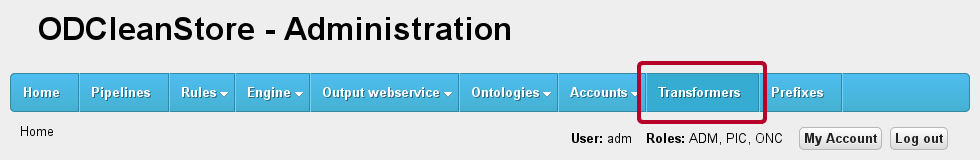
\includegraphics[width=\textwidth]{images/fe-walkthrough-menu-transformers.png}
	\label{fig:feWTMenuTransformers}
\end{figure}
\FloatBarrier

	\item Click \quot{Add a new transformer}

\begin{figure}[!h]
    \centering
    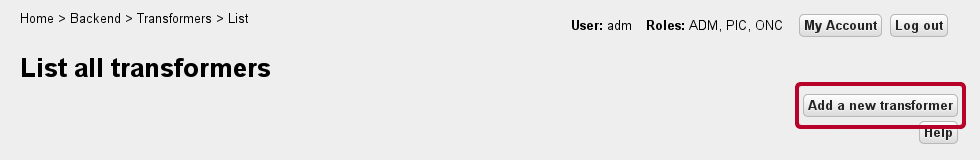
\includegraphics[width=\textwidth]{images/fe-walkthrough-add-transformer.png}
	\label{fig:feWTAddTransformer}
\end{figure}
\FloatBarrier

	\item Fill in label of your choice
	
	\item Describe its purpose
	
	\item Select the path to the backend JAR
	
	\item Fill in the classname
	
\begin{figure}[!h]
    \centering
    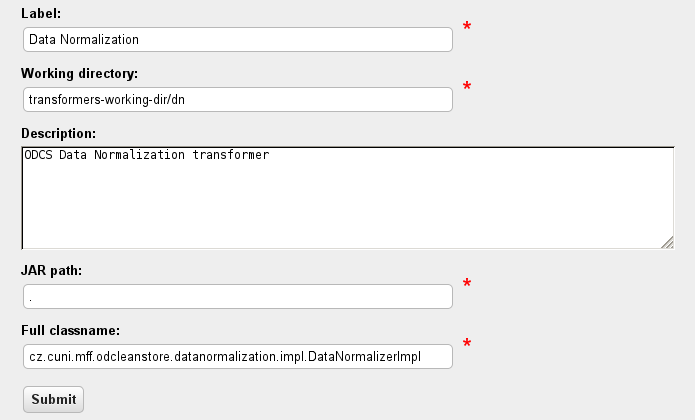
\includegraphics[width=\textwidth]{images/fe-walkthrough-new-transformer.png}
	\label{fig:feWTNewTransformers}
\end{figure}
\FloatBarrier

\end{enumerate}

\subsection*{Prepare Rules for Standard Transformer}
\begin{enumerate}[resume]
	\item Choose \code{Rules/Data Normalization} from the frontend menu

\begin{figure}[!h]
    \centering
    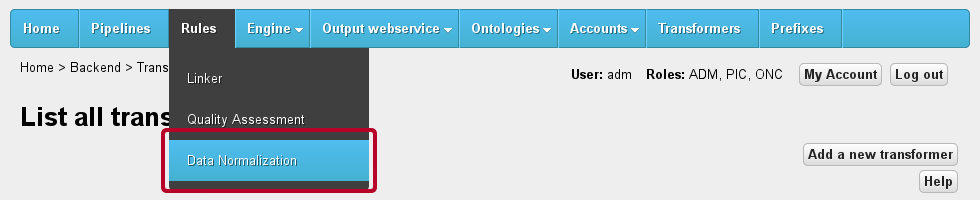
\includegraphics[width=\textwidth]{images/fe-walkthrough-menu-rules.png}
	\label{fig:feWTMenuRules}
\end{figure}
\FloatBarrier

	\item Click \quot{Add a new rules group}

\begin{figure}[!h]
    \centering
    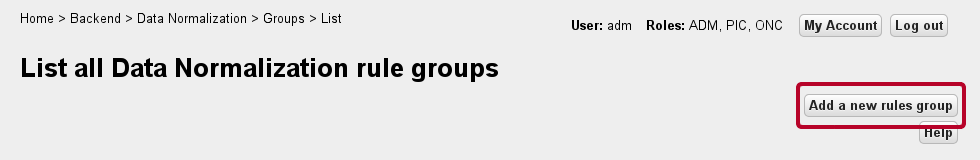
\includegraphics[width=\textwidth]{images/fe-walkthrough-add-group.png}
	\label{fig:feWTAddGroup}
\end{figure}
\FloatBarrier

	\item Fill in necessary information and submit it

\begin{figure}[!h]
    \centering
    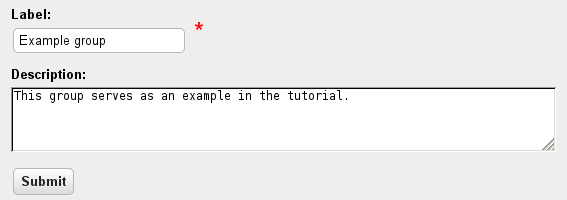
\includegraphics[width=\textwidth]{images/fe-walkthrough-new-group.png}
	\label{fig:feWTNewGroup}
\end{figure}
\FloatBarrier

	\item Click \quot{Add a new raw rule}

\begin{figure}[!h]
    \centering
    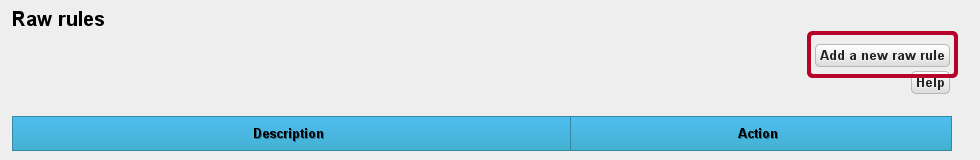
\includegraphics[width=\textwidth]{images/fe-walkthrough-add-raw-rule.png}
	\label{fig:feWTAddRawRule}
\end{figure}
\FloatBarrier

	\item Fill in its description and submit

\begin{figure}[!h]
    \centering
    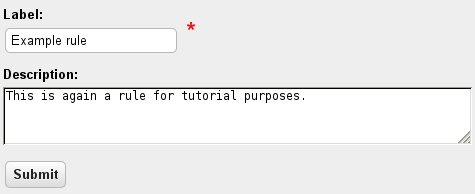
\includegraphics[width=\textwidth]{images/fe-walkthrough-new-raw-rule.png}
	\label{fig:feWTNewRawRule}
\end{figure}
\FloatBarrier

	\item Click \quot{Add a new rule component}

\begin{figure}[!h]
    \centering
    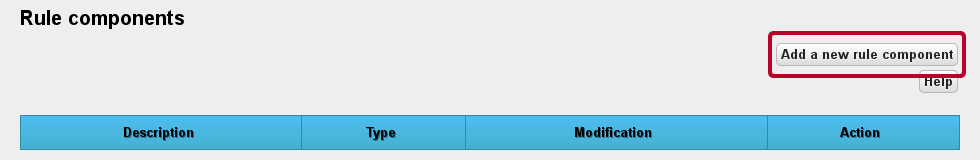
\includegraphics[width=\textwidth]{images/fe-walkthrough-add-component.png}
	\label{fig:feWTAddComponent}
\end{figure}
\FloatBarrier

	\item Choose the type of the data transformation (\code{MODIFY}/\code{INSERT}/\code{DELETE})
	\item Specify the triples that will modify the graph
	\item Describe the meaning of this transformation and submit it

\begin{figure}[!h]
    \centering
    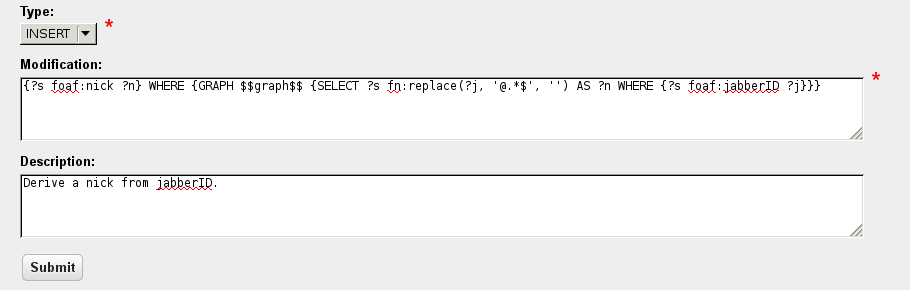
\includegraphics[width=\textwidth]{images/fe-walkthrough-new-component.png}
	\label{fig:feWTNewComponent}
\end{figure}
\FloatBarrier

	\item Repeat until the rule is complete
\end{enumerate}

  
\subsection*{Prepare Pipeline}
\begin{enumerate}[resume]
	\item Click \quot{Add a new pipeline}, fill in the label and description and submit it

\begin{figure}[!h]
    \centering
    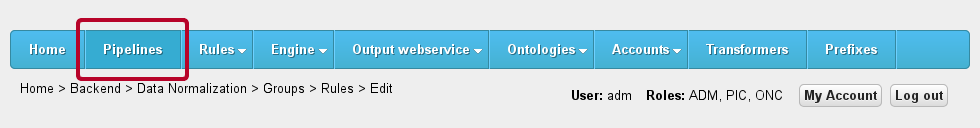
\includegraphics[width=\textwidth]{images/fe-walkthrough-menu-pipelines.png}
	\label{fig:feWTMenuPipelines}
\end{figure}
\FloatBarrier

	\item Click \quot{Assign a transformer}

\begin{figure}[!h]
    \centering
    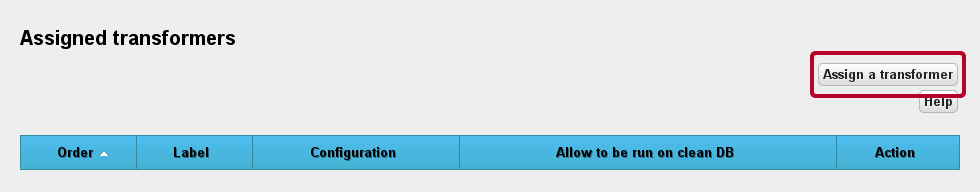
\includegraphics[width=\textwidth]{images/fe-walkthrough-assign-transformer.png}
	\label{fig:feWTAssignTransformer}
\end{figure}
\FloatBarrier

	\item Select one of the transformers
	
	\emph{If there is no option then go back to the} \textbf{\nameref{sec:prepareTransformer}} \emph{section}
	
	To be able to assign rule groups select one of the standard transformers (QualityAssessor, DataNormalizer, Linker)

	\item Fill in the configuration needed by the transformer
	\item Allow or disallow running on clean DB
	\item Select place in the pipeline

\begin{figure}[!h]
    \centering
    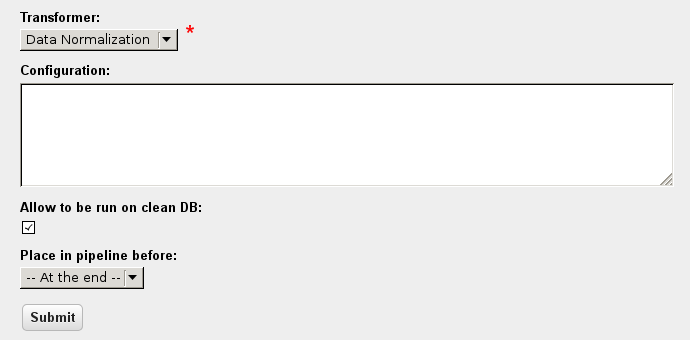
\includegraphics[width=\textwidth]{images/fe-walkthrough-new-transformer-assignment.png}
	\label{fig:feWTNewTransformerAssignment}
\end{figure}
\FloatBarrier

	\item Click \quot{Assign a group} to assign a group of Data Normalization rules

\begin{figure}[!h]
    \centering
    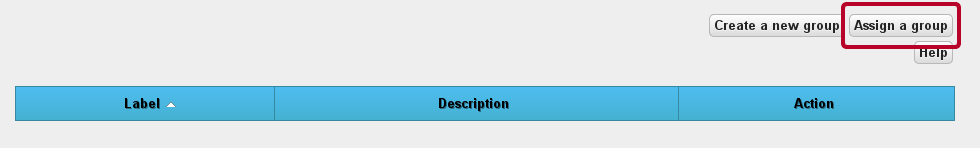
\includegraphics[width=\textwidth]{images/fe-walkthrough-assign-group.png}
	\label{fig:feWTAssignGroup}
\end{figure}
\FloatBarrier

	\item Select the group created earlier

\begin{figure}[!h]
    \centering
    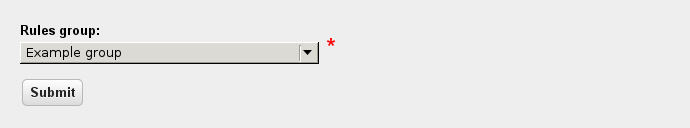
\includegraphics[width=\textwidth]{images/fe-walkthrough-new-group-assignment.png}
	\label{fig:feWTNewGroupAssignment}
\end{figure}
\FloatBarrier

\end{enumerate}

%%%%%%%%%%%%%%%%%%%%%%%%%%%%%%%%%%%%%%%%%%%%%%%%%%%%%%%%%%%%%%%%%%%%%%%%%%%%%%

\chapter{Web Services}
\section{Web Services Overview}
ODCleanStore communicates with third-party applications via webservices. Data producers can store data to ODCleanStore through \term{Input Webservice}, while data consumers may use \term{Output Webservice} to query the stored \& processed data. In addition, stored data can be accessed through a~public SPARQL endpoint. Input Webservice requires authorization, Output Webservice and the SPARQL endpoint do not.

\section{Data Producer}
\label{sec:inputWS}

New data can be stored to ODCleanStore through Input Webservice, a~SOAP multithreaded webservice that accepts RDF data serialized as RDF/XML\footnote{\url{http://www.w3.org/TR/rdf-syntax-grammar/}} or TTL\footnote{TTL or Turtle -- Terse RDF Triple Language; \url{http://www.w3.org/TeamSubmission/turtle/}} and additional metadata. The webservice requires authorization with a~valid user name and password.

The location of Input Webservice can be configured by the \code{input\_ws.endpoint\_url} configuration option (see \refadminmanual); by default, it is:
\begin{center}
\varcode{host}\code{:8080/inputws}
\end{center}

See Section \ref{sec:inputProcessing} for more information about how the inserted data are processed and stored.

\subsection{Request parameters}
\label{sec:inputWSParams}

Table \ref{tbl:inputWSParams} enumerates parameters of Input Webservice. All the parameters are required.

\begin{table}[h!]
\centering
\begin{tabular}{|l|l|l|}
	\hline
	Name & Description & Type \\
	\hline \hline
	\code{user} & user login name & \vartext{string}  \\
	\hline
	\code{password} & user password  & \vartext{string} \\
	\hline
	\code{payload} & data to insert serialized as RDF/XML or TTL & \vartext{string} \\
	\hline
	\code{metadata} & metadata about \code{payload} & see Table \ref{tbl:inputWSMetadata} \\
	\hline
\end{tabular}
\caption{Input Webservice parameters}
\label{tbl:inputWSParams}
\end{table}

\subsubsection{Metadata}
Table \ref{tbl:inputWSMetadata} lists fields that the \code{metadata} parameter consists of.

\begin{table}[h!]
\centering
\begin{tabularx}{\textwidth}{|l|X|p{2.2cm}|c|}
	\hline
	Name & Description & Type & Cardinality\\
	\hline \hline
	\code{uuid} & UUID string unique for the current request & UUID & 1 \\
	\hline
	\code{dataBaseUrl} & base URI for resolution of relative URIs in \code{payload} & URI & 1 \\
	\hline
	\code{source} & location of where the data were retrieved from & URI & 1..* \\
	\hline
	\code{publishedBy} & identifier(s) of the publisher(s) of the data & URI & 1..* \\
	\hline
	\code{license} & license(s) under which the data are published & URI & 0..* \\
	\hline
	\code{provenance} & additional provenance metadata serialized as RDF/XML or TTL & RDF/XML\newline or TTL & 0..1 \\
    \hline
	\code{pipelineName} & identifier of the pipeline that should process the inserted data & \vartext{string} & 0..1  \\
	\hline
	\code{updateTag} & distinguisher of set of graphs that update each other & \vartext{string} & 0..1  \\
	\hline
\end{tabularx}
\caption{Input Webservice \code{metadata} fields}
\label{tbl:inputWSMetadata}
\end{table}


Each request is identified by a~unique UUID generated on the client side and sent in the \code{uuid} field.
The client side is responsible for generating different UUIDs for new requests.
UUID doesn't change during the whole message transfer nor in case of a~repeated request after an exception.
\todo{PJ: popsat proč a jak; doplnit popis odolnosti vůči vícenásobným uuid}

The \code{dataBaseUrl} field is the base URI for \code{payload}.

The \code{source} field is a~list or URIs the data were retrieved from. Typically, this would be URI(s) of webpage(s) the data were scraped from but in general it can be any URI.

The \code{publishedBy} field is a~list of URIs representing the publisher of the data. It can be a~well known URI, or, for example, the host part of the source URI (e.g. \linebreak[4]\code{http://en.wikipedia.org/} for data scraped from the English Wikipedia).

The \code{license} field may specify URI(s) representing the license(s) under which \code{payload} contents and any additional  metadata being inserted are published. 

The optional \code{provenance} field can contain additional RDF provenance metadata about contents of \code{payload}.\footnote{The suggested vocabulary for these purposes is W3P (\url{http://code.google.com/p/od-w3p/}).} Base URI for the provenance metadata is the URI of the named graph where \code{payload} is stored in ODCleanStore.

The optional \code{pipelineName} field can contain a~string identifier of an existing pipeline in ODCleanStore that should be used to process the inserted data. If omitted, the default pipeline is used. \todo{reference na příslušnou sekci Admin manual}

The optional \code{updateTag} field serves as a distinguisher of data that update an already inserted version of data. If one named graph is to be considered an update of another named graph, both of them must have the same value of \code{updateTag}. For more information about how updates are detected, see Section \ref{sec:inputProcessing}, step \ref{item:updateDetection}.

\subsection{Exceptions}
\todo{PJ: nejsem si jistý, jak u WS výjimky fungují -> upravit, aby to odpovídalo skutečnosti, doplnit a učesat}

Error during a~request to Input Webservice is indicated by throwing an exception. Table \ref{tbl:inputWSExceptions} summarizes exceptions that can occur. In case of such exception, no data or \code{uuid} value for the interrupted request are stored.

\todo{PJ: jak se indikuje úspěch?}

\begin{table}[h!]
\centering
\begin{tabularx}{\textwidth}{|l|c|X|}
	\hline
	Exception & Code & Description \\
	\hline \hline
	SERVICE\_BUSY & 1 & Service busy -- occurs when maximum limit of concurrent connections is exceeded \\
	\hline
	BAD\_CREDENTIALS & 2 & Bad credentials (invalid \code{user} or \code{password}) \\
	\hline
	NOT\_AUTHORIZED & 3 & Not authorized -- user doesn't have SCR role \mbox{assigned} \\
	\hline
	DUPLICATED\_UUID & 4 & Duplicate uuid -- another request with the same \code{uuid} value has already successfully finished\\
	\hline
	UUID\_BAD\_FORMAT & 5 & Wrong format of the \code{uuid} field\\
	\hline
	UNKNOWN\_PIPELINENAME & 6 & No pipeline with name as given in \code{pipelineName} \mbox{exists} \\
	\hline
	OTHER\_ERROR & 7 & Other error; when a~new transmission with the same \code{uuid} as the current \code{uuid} is started before the current transmission finishes, OTHER\_ERROR is thrown; only the new transmission will continue \\
	\hline
	FATAL\_ERROR & 8 & Fatal error\\
	\hline
	METADATA\_ERROR & 9 & Invalid metadata -- a~field has a~wrong format or a~required field is missing \\
	\hline
\end{tabularx}
\caption{Input Webservice exceptions}
\label{tbl:inputWSExceptions}
\end{table}

\FloatBarrier

\subsection{Java API}
Third-party applications can access Input Webservice directly, or use the Java client library provided in ODCleanStore distribution. \todo{location on the CD}
Add \code{odcs-inputclient-}\textit{version}\code{.jar} library to your project and use class \code{OdcsService} to access Input Webservice programmatically.

\lstlistingname~\ref{lst:clientLibrary} gives an example of how the client library can be used.

\begin{lstlisting}[caption={Example usage of Input Webservice client library},label=lst:clientLibrary]
try {
  File payloadFile = new File("data.rdf");

  final int BUFFER_SIZE = 1024 * 4;
  char[] buffer = new char[BUFFER_SIZE];
  int count = 0;
  StringBuilder  provenancePayload = new StringBuilder();
  InputStreamReader provenanceReader = new InputStreamReader(
          new FileInputStream("provenance-metadata.rdf"), "UTF-8");
  while (-1 != (count = provenanceReader.read(buffer, 0, BUFFER_SIZE))) {
      provenancePayload.append(buffer, 0, count);
  }
  provenancePayload.close();

  Metadata metadata = new Metadata(UUID.randomUUID());
  metadata.setDataBaseUrl(new URI("http://en.wikipedia.org/wiki/Berlin"));
  metadata.getSource().add(new URI("http://en.wikipedia.org/wiki/Berlin"));
  metadata.getPublishedBy().add(new URI("http://en.wikipedia.org"));
  metadata.getLicense().add(new URI("http://creativecommons.org/licenses/by-sa/3.0/")); 
  metadata.setPipelineName("examplePipeline");
  metadata.setUpdateTag("example"); 
  metadata.setProvenance(provenancePayload.toString()); 

  OdcsService service = new OdcsService("http://localhost:8088/inputws");
  service.insert("username", "password", metadata, payloadFile, "UTF-8");
} catch (Exception e) {
  e.printStackTrace();
}
\end{lstlisting}

\section{Data Consumer}
\label{sec:outputWS}

A consumer of data stored in ODCleanStore can query the database through Output Webservice. The Output Webservice can be queried for data about a~given URI resource, queried by keywords, queried for contents of a~given named graphs or queried for metadata of a~named graph. Conflicts in data returned in response to a~query are resolved and the data are fused using policies provided by the user or by the administrator.

Additionally, the user can access the data in the clean database directly using the SPARQL endpoint powered by Virtuoso.\footnote{\url{http://virtuoso.openlinksw.com/}} This way the data consumer can use the full power of the SPARQL query language, however conflict resolution and provenance tracking is not supported for this type of queries.

\todo{specify where the SPARQL endpoint can be accessed, link to Virtuoso documentation; mention it is read-only}

\section*{Output Webservice}

The Output Webservice is a~REST webservice which can be accessed using both GET and POST HTTP methods equivalently. The port where the webservice resides can be configured by the \code{output\_ws.port} configuration option (see \refadminmanual); by default, it is on port \code{8087}.

\subsection{Types of queries}

The Output Webservice can be queried for:

\begin{enumerate}
	\item a~resource URI -- \term{URI query}
	\item keyword(s) -- \term{keyword query}
	\item named graph contents -- \term{named graph query}
	\item named graph metadata -- \term{metadata query}
\end{enumerate}

Table \ref{tbl:queryTypes} lists where each type of query can be accessed by default. The exact address can be configured.

\begin{table}[htpb]
\centering
\begin{tabularx}{\textwidth}{|l|l|X|}
	\hline
	Query & URI & Example of a~query \\
	\hline \hline
	URI & \varcode{host}\code{/uri} & \mbox{http://localhost:8087/uri} \mbox{?uri=http\%3A\%2F\%2Fexample.com} \\
	\hline
	Keyword & \varcode{host}\code{/keyword} & http://localhost:8087/keyword?kw=keyword\\
	\hline
	Named graph & \varcode{host}\code{/namedGraph} & http://localhost:8087/namedGraph \mbox{?uri=http\%3A\%2F\%2Fexample.com}\\
	\hline
	Metadata & \varcode{host}\code{/metadata} & \mbox{http://localhost:8087/metadata} \mbox{?uri=http\%3A\%2F\%2Fexample.com} \\
	\hline
\end{tabularx}
\caption{Types of queries}
\label{tbl:queryTypes}
\end{table} 

More information is available in the Query Execution specification. \todo{reference}

\subsection{Request format}

Table \ref{tbl:requestFormatUK} lists (either GET or POST) parameters than can be used with the URI, keyword and named graph queries. The \code{uri} parameter is required for URI query, \code{kw} parameter for keyword query. Other parameters are optional.

\begin{table}[htpb]
\centering
\begin{tabularx}{\textwidth}{|l|X|p{2cm}|p{2cm}|}
	\hline
	Name & Description & Possible values & Default value \\
	\hline \hline
	\code{uri} & searched URI; \newline \textit{used only with URI and named graph query} & \vartext{string} & \vartext{N/A} \\
	\hline
	\code{kw} & searched keyword(s); \newline \textit{used only with keyword query} & \vartext{string} & \vartext{N/A} \\
	\hline
	\code{format} & format of the response & \code{html}, \code{trig}, \code{rdfxml} & \code{html} \\
	\hline
	\code{aggr} & default aggregation method & \vartext{string} & \code{ALL} \\
	\hline
	\code{es} & error strategy -- handling of values for which aggregation fails & \code{IGNORE}, \code{RETURN\_ALL} & \code{RETURN\_ALL} \\
	\hline
	\code{multivalue} & default multivalue setting & 0, 1 & 0 \\
	\hline
	\code{paggr[\vartext{property}]} & aggregation method for the given \mbox{property};  example:

	  \code{paggr[rdfs\%3Alabel]=ANY} & \vartext{string} & \vartext{N/A} \\
	\hline
	\code{pmultivalue[\vartext{property}]} & multivalue setting for the given \mbox{property}; example:

	  \code{pmultivalue[rdf\%3Atype]=1} & 0, 1 & \vartext{N/A} \\
	\hline
\end{tabularx}
\caption{URI, keyword and named graph query parameters}
\label{tbl:requestFormatUK}
\end{table} 

Table \ref{tbl:requestFormatNG} lists parameters that can be used with the metadata query.

\begin{table}[htp]
\centering
\begin{tabular}{|l|l|l|l|l|}
	\hline
	Name & Description & Possible values & Default value & Required \\
	\hline \hline
	\code{uri} & URI of the requested named graph & \vartext{string} & \vartext{N/A}  & yes\\
	\hline
	\code{format} & format of the result & \code{html}, \code{trig}, \code{rdfxml} & \code{html} & no \\
	\hline
\end{tabular}
\caption{Metadata query parameters}
\label{tbl:requestFormatNG}
\end{table}

For all queries, parameters and values are case-sensitive. Property names may be either full URIs, or prefixed names (e.g. \code{rdfs:label}). Available prefixes are managed in the administration frontend (see section \ref{sec:frontendPrefixMgmt}).

For more information about aggregation settings, see the corresponding section of Conflict Resolution specification\todo{reference}.

%\newpage % just for the tables to fit better

\FloatBarrier

\subsubsection*{General aggregation methods}

\enumtable
{
	ALL & returns all conflicting values \\
	BEST & value with the highest aggregated quality; in case of equality, the newest timestamp is preferred \\
	LATEST & value with the newest timestamp; in case of equality, the highest aggregate quality is preferred \\
	ANY & returns a~single arbitrary value \\
	CONCAT & concatenation of conflicting values separated by \quot{\code{;\ }} \\
	NONE & returns all conflicting values including duplicities
}

\subsubsection*{Numeric aggregation methods}

\enumtable
{
	MIN & minimum of conflicting values \\
	MAX & maximum of conflicting values \\
	AVG & average of conflicting values \\
	MEDIAN & median of conflicting values
}

\subsubsection*{Date aggregation methods}

\enumtable
{
	MIN & the earliest date \\
	MAX & the latest date
}

\subsubsection*{String aggregation methods}

\enumtable
{
	SHORTEST & the shortest string \\
	LONGEST & the longest string
}

\subsubsection*{Error strategy}
The error strategy determines how to handle values that cannot be aggregated by the given aggregation method, e.g. when applying MEDIAN aggregation to a~mix of numeric and date values.

Note that for some aggregations, an untyped literal may be converted to a~numeric literal (\code{xsd:double}) if possible.

\subsubsection*{Multivalue parameter}
The multivalue parameter determines whether differences with other conflicting values decrease quality (\code{multivalue=0}), or not (\code{multivalue=1}). Setting multivalue to false (0) is appropriate for properties with a~single value (e.g. \code{dbprop:population}), setting it to true (1) is appropriate for propertiees with multiple possible values (e.g. \code{rdf:type}).

\todo{content-negotiation}

\subsection{Query Format}

\subsubsection{URI Query}
The value of the \code{uri} parameter must be either a~full valid URI, or a~prefixed name (e.g. \code{dbpedia:Berlin}).  Available prefixes are managed in the administration frontend (see section \ref{sec:frontendPrefixMgmt}).

\subsubsection{Keyword Query}
The \code{kw} parameter can contain one or more keywords separated by whitespace. If a~keyword itself contains spaces, it may be enclosed in double quotes. Query Execution looks for literals that contain all of the keywords. Keywords can also contain the \code{*} wildcard, but they must begin with at least four non-wildcard characters if a~wildcard is to be used.

Query Execution also looks for an exact match of the entire \code{kw} value (i.e. without any division to keywords). If the \code{kw} value is a~number, then numeric typed literals will also match; if the \code{kw} value is formatted as \code{xsd:dateTime}\footnote{\url{http://www.w3.org/TR/xmlschema-2/\#dateTime-lexical-representation}}, then \code{xsd:dateTime} typed literals will also match.

Special characters, such as quotes and backslashes may be filterd out from searched keyword(s).

\subsubsection{Named Graph Query}
The value of the \code{uri} parameter must be either a~valid URI, or a prefixed name, of an existing named graph.

\subsubsection{Metadata Query}
The value of the \code{uri} parameter must be a~valid URI of an existing named graph.

\subsection{Results Format for URI \& Keyword Queries}
\label{sec:URIKWResultsFormat}

The result contains triples returned in response to the query, including relevant labels of URI resources in the result, and metadata for the triples.

\subsubsection{HTML}

The result in HTML format contains results in a~human-readable form (\figurename~\ref{fig:uriQuery}). It contains

\begin{itemize}
	\item a~table with all triples in the result together with their aggregated quality and named graphs from which the triple was selected or calculated,
  \item  a~table with metadata of named graphs occuring in the first table.
\end{itemize}

\begin{figure}[htb]
    \centering
    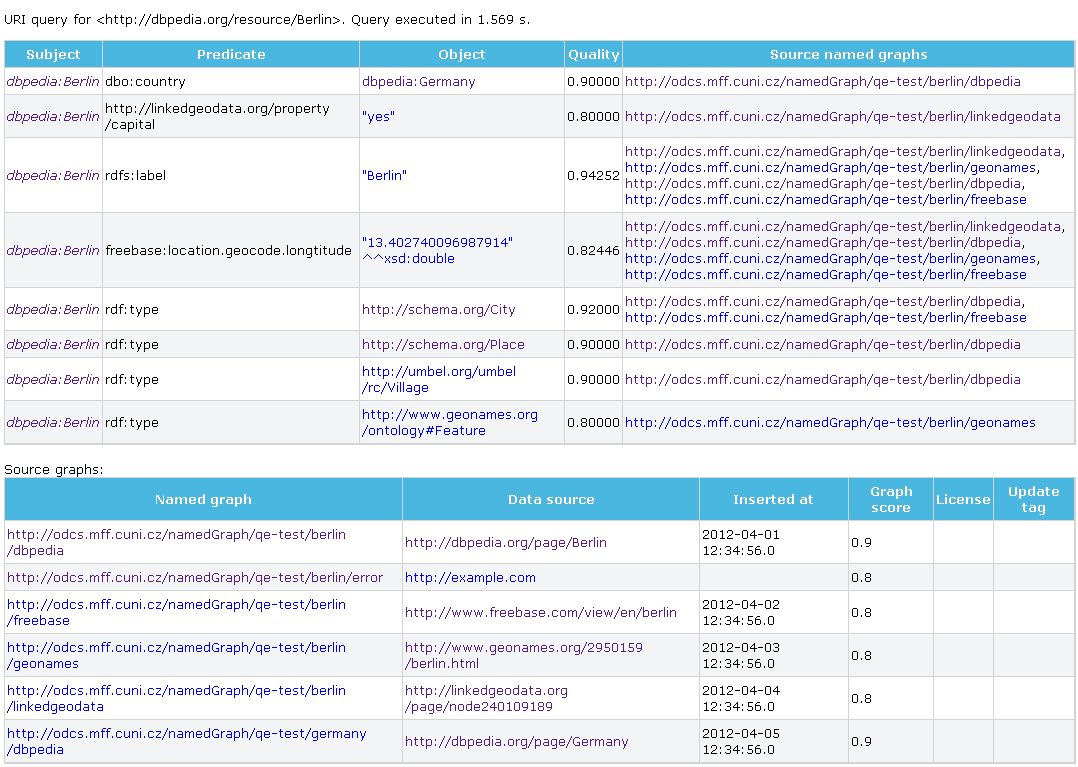
\includegraphics[width=\textwidth]{images/uri-query-screenshot.png}
    \caption{Example of HTML output for URI query for \code{dbpedia:Berlin}}
	\label{fig:uriQuery}
\end{figure}

\subsubsection{TriG}
\label{sec:URIKWTrig}

If the \code{format} parameter is set to \code{trig}, the result contains triples (quads) serialized in the TriG\footnote{\url{http://www4.wiwiss.fu-berlin.de/bizer/trig/}} format. The result includes:

\begin{itemize}
	\item triples returned in response to the query, each one placed in a~unique named graph
  \item aggregated quality (\code{odcs:quality}) and source named graphs (\code{odcs:sourceGraph}) of the above triples; subjects of these statements are the unique named graphs where the respective triples are placed
  \item  metadata of source named graphs; they may include where the data were extracted from (\code{w3p:source}), Quality Assesment score of the named graph (\code{odcs:score}) and of its publisher (\code{odcs:publisherScore}), the publisher of the data (\code{w3p:publishedBy}), timestamp (\code{w3p:insertedAt}), license (\code{dc:license}), update tag (\code{odcs:updateTag})
  \item  metadata about the query response itself -- a~title (\code{dc:title}), date (\code{dc:date}), number of result triples (\code{odcs:totalResults}), the query (\code{odcs:query}) and link to each result item (\code{odcs:result})
\end{itemize}

\pagebreak[3]

An example:

\begin{lstlisting}[caption={Example of URI or keyword query response in TriG},label=lst:URIKWTrigResponse]
@prefix :        <#> .
@prefix odcs:    <http://opendata.cz/infrastructure/odcleanstore/> .
@prefix w3p:     <http://purl.org/provenance#> .
@prefix rdfs:    <http://www.w3.org/2000/01/rdf-schema#> .
@prefix rdf:     <http://www.w3.org/1999/02/22-rdf-syntax-ns#> .
@prefix dcterms: <http://purl.org/dc/terms/> .
@prefix dbpedia: <http://dbpedia.org/ontology/> .

<http://opendata.cz/infrastructure/odcleanstore/query/results/1> {
  <http://dbpedia.org/resource/Berlin> rdfs:label "Berlin"@en .
}

<http://opendata.cz/infrastructure/odcleanstore/query/results/2> {
  <http://dbpedia.org/resource/Berlin> dbpedia:populationTotal
    "3420768"^^<http://www.w3.org/2001/XMLSchema#int> .
}

<http://opendata.cz/infrastructure/odcleanstore/query/metadata/> {
  <http://opendata.cz/infrastructure/odcleanstore/query/results/1>
    odcs:quality 0.92 ;
    w3p:source <http://opendata.cz/infrastructure/odcleanstore/data/e0cdc9d7-e2d8-4bde> ;
    w3p:source <http://opendata.cz/infrastructure/odcleanstore/data/b68e21f7-363f-4bfd> .

  <http://opendata.cz/infrastructure/odcleanstore/query/results/2>
    odcs:quality 0.8966325468133597 ;
    w3p:source <http://opendata.cz/infrastructure/odcleanstore/data/b68e21f7-363f-4bfd> .

  <http://opendata.cz/infrastructure/odcleanstore/data/e0cdc9d7-e2d8-4bde>
    odcs:score 0.9 ;
    w3p:insertedAt "2012-04-01 12:34:56.0"^^<http://www.w3.org/2001/XMLSchema#dateTime> ;
    w3p:source <http://dbpedia.org/page/Berlin> ;
    w3p:publishedBy <http://dbpedia.org/> ;
    dcterms:license <http://creativecommons.org/licenses/by-sa/3.0/> ;
    odcs:publisherScore 0.9 ;
    odcs:updateTag "dataset123".
	

  <http://opendata.cz/infrastructure/odcleanstore/data/b68e21f7-363f-4bfd>
    odcs:score 0.8 ;
    w3p:insertedAt "2012-04-04 12:34:56.0"^^<http://www.w3.org/2001/XMLSchema#dateTime> ;
    w3p:source <http://linkedgeodata.org/page/node240109189> .

  <http://localhost:8087/uri?uri=http%3A%2F%2Fdbpedia.org%2Fresource%2FBerlin>
    a odcs:QueryResponse ;
    dc:title "URI search: http://dbpedia.org/resource/Berlin" ;
    dc:date "2012-08-01T10:20:30+01:00" ;
    odcs:totalResults 2 ;
    odcs:query "http://dbpedia.org/resource/Berlin" ;
    odcs:result <http://opendata.cz/infrastructure/odcleanstore/query/results/1> ;
    odcs:result <http://opendata.cz/infrastructure/odcleanstore/query/results/2> .
}
\end{lstlisting}

\subsubsection{RDF/XML}
\label{sec:URIKWRDFXML}

If the \code{format} parameter is set to \code{rdfxml}, then the result will be formatted in RDF/XML.\footnote{\url{http://www.w3.org/TR/REC-rdf-syntax/}} The returned triples contain

\begin{itemize}
  \item triples returned in response to the query,
  \item  metadata about the query response itself
\end{itemize}

as in case of TriG output, however no metadata about quality of triples or about source named graphs are included.

\subsubsection{Paging of results}
\label{sec:URIKWPaging}
As of now, all results are returned on a single page. The approximate maximum number of triples in the result is 500 by default (and can be set in the configuration file, see \refadminmanual).

\subsection{Results Format for Named Graph Query}
Named graph query selects all triples stored in the given named graph and is intended mainly for debugging purposes.
The format of results for the named graph query is exactly the same as for URI or keyword queries (see Section~\ref{sec:URIKWResultsFormat}). The only difference is that labels for URI resources in the result are not retrieved (unless they are contained in the named graph). Also, conflict resolution considers only the named graph and not any other conflicting (or same) values that may be stored in other graphs.

\subsection{Results Format for Metadata Query}
The result contains metadata and Quality Assessment results for a given named graph. The metadata include metadata maintained by ODCleanStore (e.g. \code{odcs:insertedAt}) and data from the \code{provenance} metadata graph. Quality Assessment is executed on the named graph at query time, with rules that would be applied to it in its respective pipeline.

\subsubsection{HTML}

The result in HTML format contains results in a~human-readable form (\figurename~\ref{fig:metadataQuery}). It contains

\begin{itemize}
  \item a table with ODCleanStore metadata,
  \item the results of Quality Assessment, i.e. the resulting score and all Quality Assessment rules the named graph violated and thus its score was decreased by the respective coefficient (only if there is at least one Quality Assessment rule group applicable to the named graph),
  \item \code{provenance} metadata, if available.
\end{itemize}

\begin{figure}[htb]
    \centering
    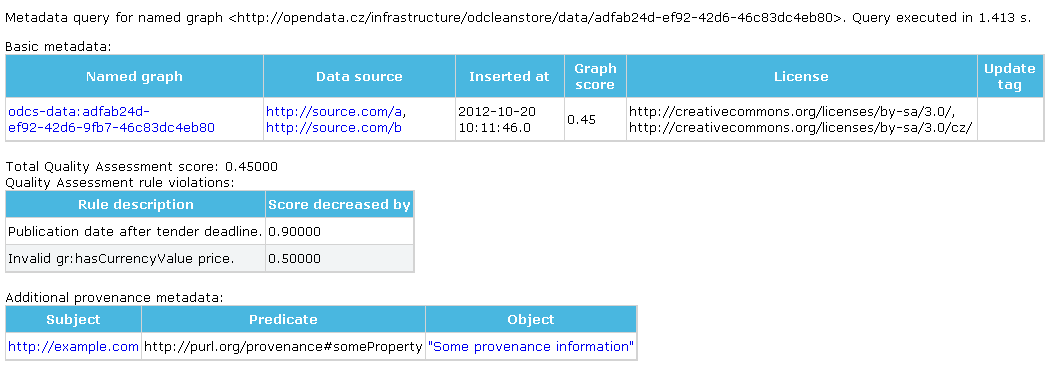
\includegraphics[width=\textwidth]{images/metadata-query-screenshot.png}
    \caption{Example of HTML output for metadata query}
	\label{fig:metadataQuery}
\end{figure}

\subsubsection{TriG}
\label{sec:metadataTriG}
The result contains triples (quads) serialized in the TriG format. Again, the result contains ODCleanStore metadata, additional \code{provenance} metadata, results of Quality Assessment and also metadata about the query response itself. The meaning of used predicates is as described in Section \ref{sec:URIKWTrig}.

The \code{provenance} metadata are contained in one named graph and a triple \varcode{payload-graph}-\code{odcs:provenanceMetadataGraph}-\varcode{provenance-graph} points to it; all other data are placed in another named graph.

\pagebreak[3]

An example:

\begin{lstlisting}[caption={Example of metadata query response in TriG},label=lst:metadataTrigResponse]
@prefix :        <#> .
@prefix odcs:    <http://opendata.cz/infrastructure/odcleanstore/> .
@prefix w3p:     <http://purl.org/provenance#> .
@prefix rdfs:    <http://www.w3.org/2000/01/rdf-schema#> .
@prefix rdf:     <http://www.w3.org/1999/02/22-rdf-syntax-ns#> .
@prefix dc:      <http://purl.org/dc/terms/> .

<http://opendata.cz/infrastructure/odcleanstore/query/metadata/> {
  <http://opendata.cz/infrastructure/odcleanstore/data/e0cdc9d7-e2d8-4bde>
    w3p:insertedAt "2012-04-01 12:34:56.0"^^<http://www.w3.org/2001/XMLSchema#dateTime> ;
    w3p:source <http://dbpedia.org/page/Berlin> ;
    dc:license <http://creativecommons.org/licenses/by-sa/3.0/> ;
    odcs:updateTag "dataset123" ;
    w3p:publishedBy <http://dbpedia.org/> ;
    odcs:provenanceMetadataGraph
      <http://opendata.cz/infrastructure/odcleanstore/provenanceMetadata/e0cdc9d7-e2d8-4bde>;
        
    odcs:score 0.72 ;
    odcs:violatedQARule <http://opendata.cz/infrastructure/odcleanstore/QARule/10> ;
    odcs:violatedQARule <http://opendata.cz/infrastructure/odcleanstore/QARule/20> .  

  <http://opendata.cz/infrastructure/odcleanstore/QARule/10>
    a odcs:QARule ;
    odcs:coefficient 0.8 ;
    dc:description "Procedure type ambiguous" .
        
  <http://opendata.cz/infrastructure/odcleanstore/QARule/20>
    a odcs:QARule ;
    odcs:coefficient 0.9 ;
    dc:description "Procurement contact person missing" .
        
  <http://localhost:8087/namedGraph?uri=http%3A%2F%2Fopendata.cz
      %2Finfrastructure%2Fodcleanstore%2Fdata%2Fe0cdc9d7-e2d8-4bde>
    a odcs:QueryResponse ;
    dc:title "Metadata for named graph:
      http://opendata.cz/infrastructure/odcleanstore/data/e0cdc9d7-e2d8-4bde" ;
    dc:date "2012-08-01T10:20:30+01:00" ;
    odcs:query "http://opendata.cz/infrastructure/odcleanstore/data/e0cdc9d7-e2d8-4bde";
}
    
<http://opendata.cz/infrastructure/odcleanstore/provenanceMetadata/e0cdc9d7-e2d8-4bde> {
  <http://opendata.cz/infrastructure/odcleanstore/data/e0cdc9d7-e2d8-4bde>
    w3p:provenanceMetadataProperty1 "provenanceMetadataValue1".
  <http://opendata.cz/infrastructure/odcleanstore/data/e0cdc9d7-e2d8-4bde>
    w3p:provenanceMetadataProperty2 "provenanceMetadataValue2".
}
\end{lstlisting}

\subsubsection{RDF/XML}
The result for a metadata query serialized in RDF/XML contains the same triples as in case of TriG (Section \ref{sec:metadataTriG}) except that triples are not divided into named graphs.

\subsubsection{Paging of results}
See Section~\ref{sec:URIKWPaging}.

\todo{JSON}
\todo{Error handling!}
\todo{Examples}

%%%%%%%%%%%%%%%%%%%%%%%%%%%%%%%%%%%%%%%%%%%%%%%%%%%%%%%%%%%%%%%%%%%%%%%%%%%%%%

\chapter{Stored Data}
\section{Input Processing}
\label{sec:inputProcessing}
\todo{PJ: zkontrolovat, jestli odpovida realite, a naopak, ze vse potrebne je implementovano}
When a new request is sent to Input Webservice, the stored data \& metadata go through several phases.

\begin{enumerate}

  \item First, data \& metadata are validated. \code{Payload} data and optional \code{provenance} metadata (see Section~\ref{sec:inputWSParams} \nameref{sec:inputWSParams}) should be valid RDF/XML or TTL, all required metadata fields must have the proper cardinality and valid format. An exception is thrown and the request interrupted if validation fails.

  \item If all data are valid, the request is queued, Input Webservice indicates success and the transmission successfully finishes.

  \item Engine, independently on Input Webservice, successively takes requests from the input queue and processes them. RDF data from \code{payload} are stored to a single named graph, \code{provenance} metadata to a separate named graph and other metadata to another separate named graph called \term{metadata graph}, all in the dirty (staging) database. The format of RDF triples in the metadata graph is described in Section~\ref{sec:storedDataStructure}.

  \item Because some predicates are reserved for purposes of internal metadata representation in ODCleanStore, RDF triples that contain these predicates are removed from \code{payload} and \code{provenance} named graphs. Table~\ref{tbl:reservedPredicates} lists all reserved predicates.

\begin{table}[h!]
\centering
\begin{tabular}{|l|}
	\hline 
	\code{odcs:score} \\
	\hline
	\code{odcs:publisherScore} \\
	\hline
	\code{odcs:scoreTrace} \\
	\hline
	\code{odcs:metadataGraph} \\
	\hline
	\code{odcs:provenanceMetadataGraph} \\
	\hline
	\code{odcs:sourceGraph} \\
	\hline
	\code{odcs:insertedAt} \\
	\hline
	\code{odcs:insertedBy} \\
	\hline
	\code{odcs:source} \\
	\hline
	\code{odcs:publishedBy} \\
	\hline
	\code{odcs:license} \\
	\hline
	\code{odcs:updateTag} \\
	\hline
	\code{odcs:isLatestUpdate} \\
	\hline
\end{tabular}
\caption{Reserved RDF predicates}
\label{tbl:reservedPredicates}
\end{table}
\todo{check it is up-to-date}

  \item Next, the processing pipeline is selected -- if \code{pipelineName} was present, pipeline with the given name is used, the default pipeline is used otherwise. Engine runs each transformer in the pipeline on the stored data. Transformers can modify the inserted named graphs or attach new named graphs (\term{attached named graph}). See~\refadminmanual{} for more information about transformers.

  \item \label{item:updateDetection}
    Engine runs a special (automatically added) transformer, that checks if the currently processed data are an update of data already stored in the clean database. More specifically, an inserted named graph $A$ is considered an update of named graph $B$ if and only if the following conditions hold:

	\begin{enumerate}[label=(\emph{\roman*})]
	  \item Named graphs $A$ and $B$ have the same update tag, or both have an unspecified (\code{null}) update tag.
	  \item Named graphs $A$ and $B$ were inserted by the same (SCR) user.
	  \item Named graphs $A$ and $B$ have the same set of sources in metadata.
	  \item Named graph $A$ was inserted later than named graph $B$.
	\end{enumerate}

	The \code{payload} named graph is marked as the latest version by adding a triple with predicate \code{odcs:isLatestUpdate} to the \code{metadata} graph. If the currently processed data update a named graph already stored in the clean database, this triple is removed for the older graph.

  \item If all transformers in the pipeline finish successfully, the \code{payload} graph, \code{provenance} graph, metadata graph and any new attached graphs are moved from the dirty database to the clean database, while the respective request is removed from the queue.

  \todo{popsat, co se deje, kdyz nastane chyba}

\end{enumerate}

\section{Stored Data Structure}
\label{sec:storedDataStructure}

Data originating from a single request to Input Webservice can be stored in several named graphs. RDF data given in the \code{payload} parameter are stored in one named graph (\code{payload} graph). If \code{provenance} RDF metadata are given, they are stored in another named graph (\code{provenance} graph). Other metadata (such as the source of data, timestamp, etc.) are stored in yet another named graph (\term{metadata graph}).
In addition, transformers in the respective pipeline may add more related RDF data to one or more named graphs (\term{attached graphs}), e.g. results of quality assessment, or mappings for resources in \code{payload}. 

While contents of the \code{payload}, \code{provenance} and attached graphs may be arbitrary, the metadata graph has a set structure. Table~\ref{tbl:metadataGraph} describes the structure of a metadata graph. In the table, \varcode{payload-graph} stands for the name of the respective \code{payload} graph, \varcode{provenance-graph} and \varcode{metadata-graph} analogously.


\begin{table}[h!]
\centering
\begin{tabularx}{\textwidth}{|l|p{5cm}|X|c|}
	\hline
	Subject & Predicate & Object & Cardinality\\
	\hline \hline
	\varcode{payload-graph} & \code{odcs:metadataGraph} & \varcode{metadata-graph} & 1 \\
	\hline
	\varcode{payload-graph} & \code{odcs:} \code{provenanceMetadataGraph} & \varcode{provenance-graph} & 0..1 \\
	\hline
	\varcode{payload-graph} & \code{odcs:attachedGraph} & URIs of attached graphs & 0..* \\
	\hline
	\varcode{payload-graph} & \code{odcs:insertedAt} & insertion time & 1 \\
	\hline
	\varcode{payload-graph} & \code{odcs:insertedBy} & name of the user who inserted the data & 1 \\ \todo{PJ: jmeno nebo ID?}
	\hline
	\varcode{payload-graph} & \code{odcs:source} & source of the data (values  from the \code{source} field) & 1..* \\
	\hline
	\varcode{payload-graph} & \code{odcs:publishedBy} & identifier of the publisher of the data (values  from the \code{publishedBy} field) & 1..* \\
	\hline
	\varcode{payload-graph} & \code{odcs:license} & license of the data (values from the \code{license} field) & 0..* \\
	\hline
	\varcode{payload-graph} & \code{odcs:updateTag} & distinguisher of graph updates (value from the \code{updateTag} field) & 0..1 \\
	\hline
	\varcode{payload-graph} & \code{odcs:isLatestUpdate} & 1 \newline
	  \emph{\footnotesize Present only for the latest version of data (see Section \ref{sec:inputProcessing}, step \ref{item:updateDetection})}
	 & 0..1 \\
	\hline
\end{tabularx}
\caption{RDF triples in a \code{metadata} graph}
\label{tbl:metadataGraph}
\end{table}

Note that transformers may add triples to the metadata graph too. For example, Quality Assessment adds these two triples:
\begin{itemize}
  \item \varcode{payload-graph} -- \code{odcs:score} -- \varcode{QA-score}
  \item \varcode{payload-graph} -- \code{odcs:scoreTrace} -- \varcode{QA-score-explanation}
\end{itemize}

\section{Executing Pipelines on the Clean Database}
\label{sec:pipelinesOnCleanDB}

The pipeline creator or administrator \todo{proper user role} can decide to re-run a transformer pipeline on one or more named graphs that are already in the clean database, e.g. when the respective transformer rules changed.\todo{reference to administration documentation} In that case, such named graphs are queued for processing and Engine successively runs the pipeline on each queued graph:

\begin{enumerate}
  \item First, a copy of the \code{payload}, \code{provenance}, metadata and any attached graphs is created in the dirty database.
  \item The same processing pipeline that was used when the data came through Input Webservice is run on this copy. Transformers can modify any of the graphs and attach new graphs.
	\todo{what if the pipeline fails?}
  \item In a transaction, the old version in the clean database is deleted and the processed copy (together with any new attached graphs) is moved from the dirty database to the clean database.
\end{enumerate}
%%%%%%%%%%%%%%%%%%%%%%%%%%%%%%%%%%%%%%%%%%%%%%%%%%%%%%%%%%%%%%%%%%%%%%%%%%%%%%

\appendix

\chapter{Glossary}

\section*{RDF-related}
\begin{glossarylist}
	\item[RDF] Resource Description Framework, a~language for representing information about resources in the World Wide Web\footnote{\url{http://www.w3.org/RDF/}}
	\item[RDF triple] Statement about a~resource expressed in the form of subject-predicate-object expression
	\item[URI] Uniform Resource Identifier, identifies RDF resources
	\item[Named graph] A~set of related RDF triples (RDF graph) named with a~URI\footnote{\url{http://www.w3.org/2004/03/trix/}}
	\item[RDF quad] An RDF triple plus named graph URI (subject, predicate, object, named graph)
	\item[Ontology] Representation of the meaning of terms in a~vocabulary and of their interrelationships
	\item[OWL] The Web Ontology Language\footnote{\url{http://www.w3.org/TR/owl-features/}}
	\item[SPARQL] RDF query language\footnote{\url{http://www.w3.org/TR/rdf-sparql-query/}}
	\item[RDF/XML] An XML-based serialization format for RDF graphs\footnote{\url{http://www.w3.org/TR/rdf-syntax-grammar/}}
	\item[TTL] Turtle -- Terse RDF Triple Language\footnote{\url{http://www.w3.org/TeamSubmission/turtle/}}; a~human-friendly alternative to RDF/XML 
\end{glossarylist}

\section*{Data \& Data Quality}
\begin{glossarylist}
	\item[Dirty (staging) database] Database where incoming data are stored until they are processed by a~processing pipeline (e.g. clean, linked to other data, etc.)
	\item[Clean database] Database where incoming data are stored after they are successfully processed by the respective processing pipeline; this database can be accessed using the Output Webservice
	\item[\code{Payload} graph] Named graph where the actual inserted data, given in the \code{payload} parameter of Input Webservice, are stored
	\item[\code{Provenance} graph] Named graph where additional provenance metadata, given in the \code{provenance} field of Input Web Service, are stored
	\item[Metadata graph] Named graph where other metadata about a \code{payload} graph (such as source, timestamp, license, etc.) are stored
	\item[Attached graph] Named graph attached to a \code{payload} graph by a transformer
	\item[Named graph score] Quality of a~single (\code{payload}) named graph estimated by the Quality Assesment component and stored in the database, expressed as a~number from interval [0,1]
	\item[Publisher score] Average score of named graphs from a~publisher
	\item[Aggregate quality] Quality of a~triple in the results calculated by the Conflict Resolution component during query time, expressed as a~number from interval [0,1]
\end{glossarylist}

\section*{Data Processing}
\begin{glossarylist}
	\item[Pipeline] A configurable sequence of transformers that is used to process a named graph. The pipeline to process data sent to Input Webservice can be selected explicitly, or the default pipeline is used.
	\item[Transformer] A Java class which implements the \term{Transformer} interface that and is registered in ODCleanStore Administration Frontend by an administrator.
	\item[Transformer instance (or transformer assignment)]  Assignment of a \term{transformer} to a \term{pipeline}. A single transformer can be assigned to multiple pipelines (or even to a single pipeline multiple times), thus creating multiple transformer instances.
	\item[Rule] Some transformers included in ODCleanStore can be configured in Administration Frontend by rules. Rules are grouped together to \term{rule groups}.
	\item[Rule group] A group of transformer \term{rules}. Rule groups can be assigned to transformer instances.
\end{glossarylist}

\section*{User Roles}
\begin{glossarylist}
	\item[ADM] Administrator
	\item[ONC] Ontology creator
	\item[PIC] Pipeline creator
	\item[SCR] Data producer (scraper)
	\item[USR] Data consumer
\end{glossarylist}

\chapter{List of Used XML Namespaces}

\begin{table}[h!]
\centering
\begin{tabular}{|l|l|}
	\hline
	\ttfamily
	\textrm{\textbf{Prefix}} & \textrm{\textbf{URI}} \\
	\hline\hline
	odcs & http://opendata.cz/infrastructure/odcleanstore/ \\
	\hline
	w3p & http://purl.org/provenance\# \\
	\hline
	dc & http://purl.org/dc/terms/ \\
	\hline
	rdf & http://www.w3.org/1999/02/22-rdf-syntax-ns\# \\
	\hline
	rdfs & http://www.w3.org/2000/01/rdf-schema\# \\
	\hline
	owl & http://www.w3.org/2002/07/owl\# \\
	\hline
	xsd & http://www.w3.org/2001/XMLSchema\# \\
	\hline
	dbpedia & http://dbpedia.org/resource/ \\
	\hline
	dbprop & http://dbpedia.org/property/ \\
	\hline
	skos & http://www.w3.org/2004/02/skos/core\# \\
	\hline
\end{tabular}
\caption{List of used XML namespaces}
\end{table} 

\end{document}
